Il est connu que tout triangle $ABC$ possède une aire donnée par $\frac12 \abs{ \det \big( \vect{AB} , \vect{AC} \big) }$ où $\frac12 \det \big( \vect{AB} , \vect{AC} \big)$ est l'aire algébrique de $ABC$.
Il devient naturel de définir l'aire algébrique d'un \ngone\ via celles de triangles comme dans l'exemple suivant utilisant les triangles $\Omega AB$, $\Omega BC$, $\Omega CD$, $\Omega DE$ et $\Omega EA$. A priori, le résultat pourrait dépendre du point $\Omega$ employé, mais le fait \ref{garea-pt-ct}, donné plus bas, montrera que ce n'est pas le cas.

\begin{multicols}{2}
	\small\itshape
    \begin{center}
		Calcul direct à la main.

		\smallskip

        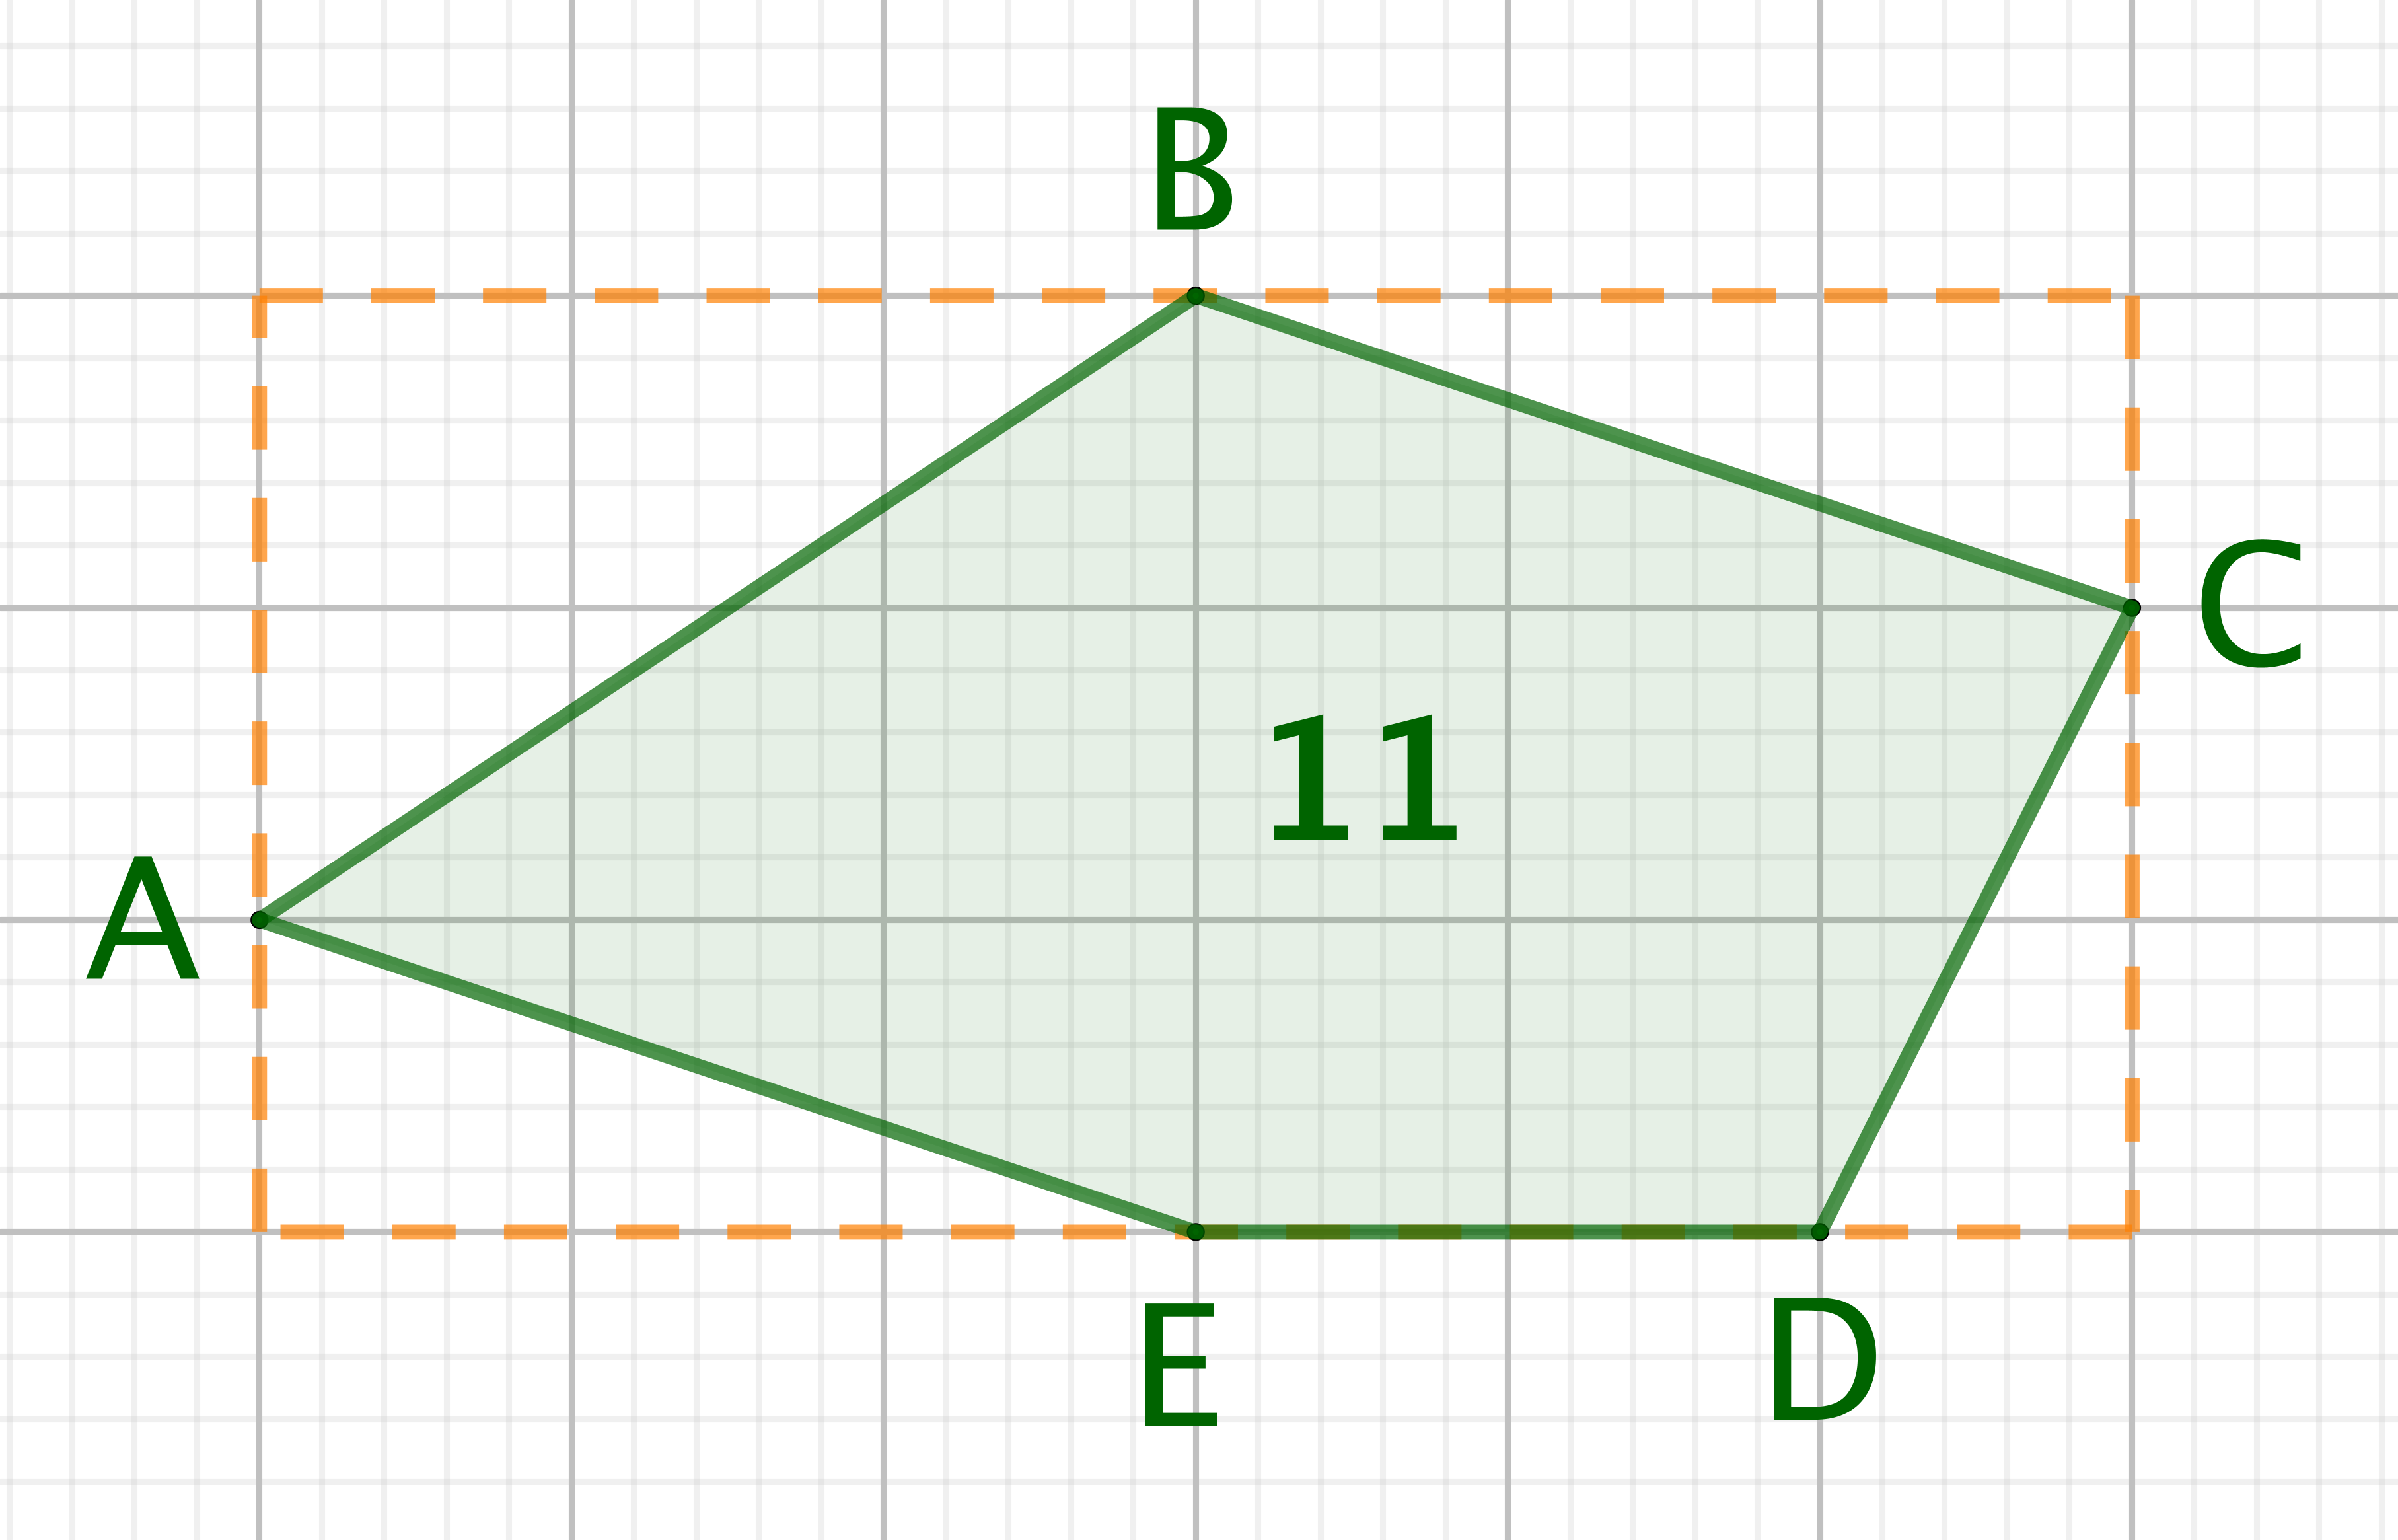
\includegraphics[scale=.35]{content/polygon/at-least-one/convex-1.png}

       	\smallskip

		$11 = 3 \cdot 6 - \dfrac{3 \cdot 1 + 3 \cdot 2 + 3 \cdot 1 + 1 \cdot 2}{2}$
    \end{center}

	\columnbreak

    \begin{center}
		Via le déterminant.

		\smallskip

        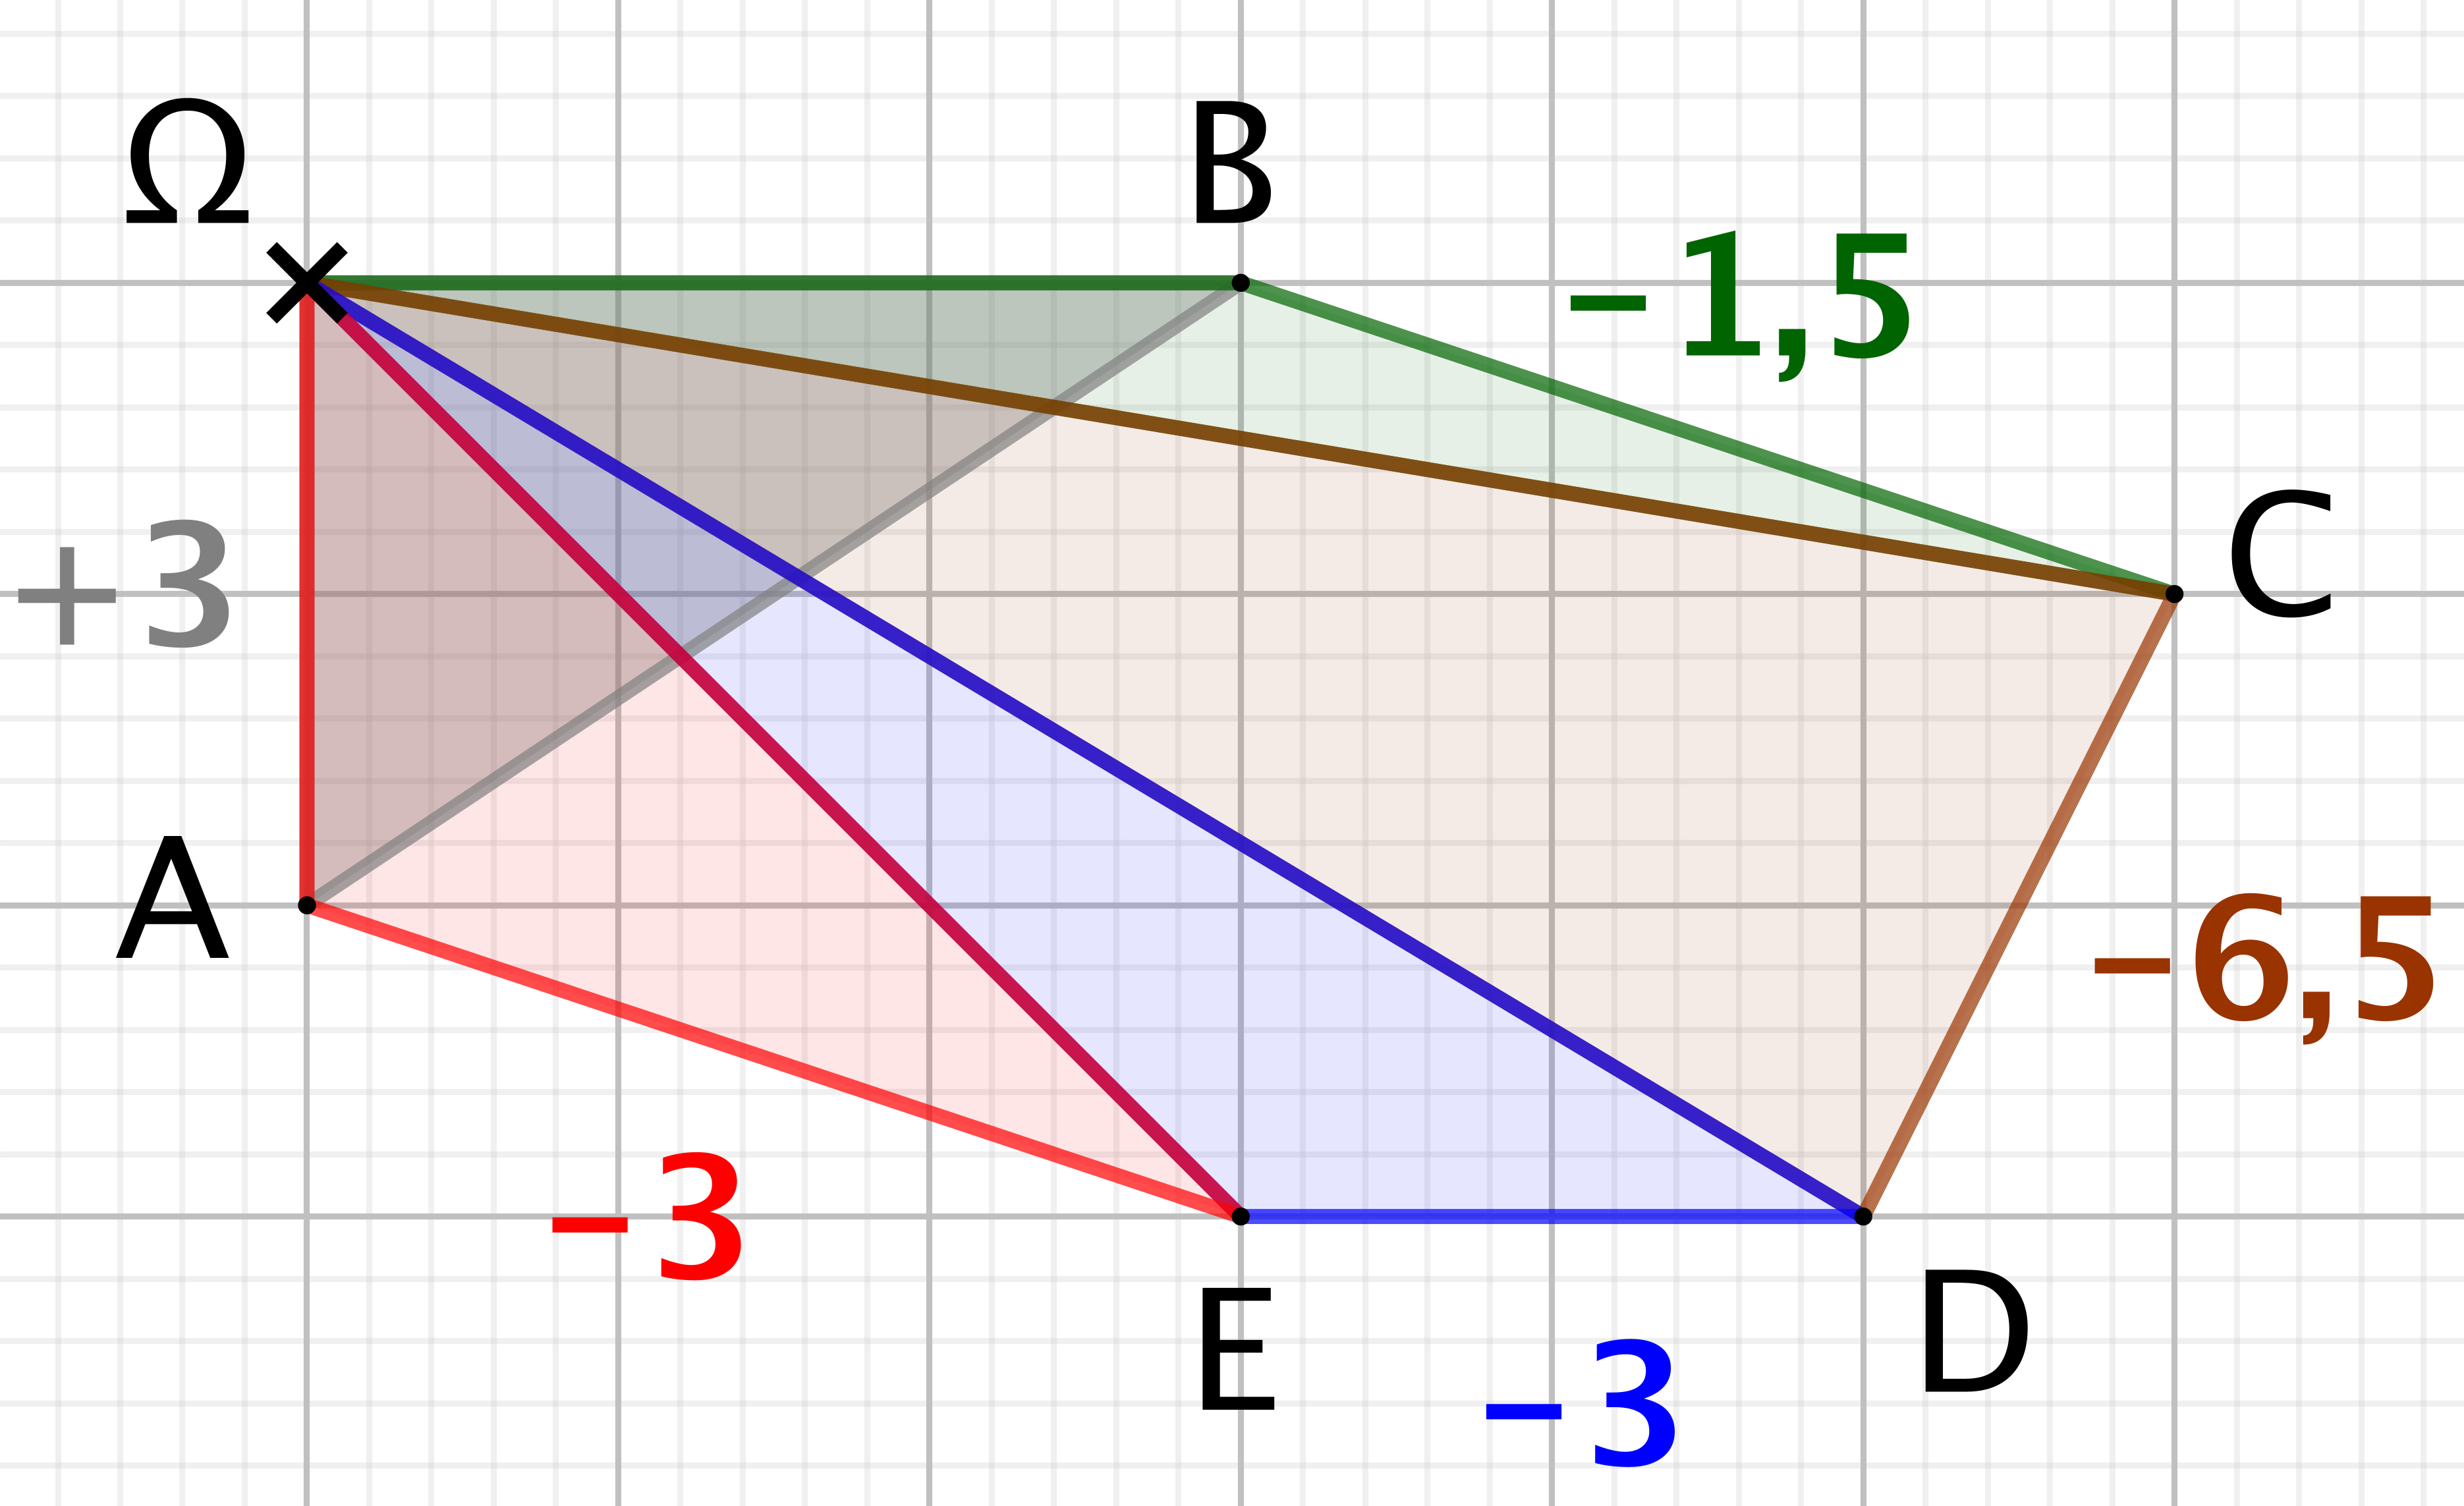
\includegraphics[scale=.35]{content/polygon/at-least-one/convex-2.png}

       	\smallskip

		$- 11 = 3 - \num{1.5} - \num{6.5} - 3 - 3 \vphantom{\dfrac22}$
    \end{center}
\end{multicols}


Ce mode de calcul est celui employé par \geogebra\ qui donne une aire de \num{6.5} pour le polygone croisé de la bande dessinée ci-après qui détaille les calculs faits: les aires algébriques représentées en bleu sont positives, et celles en rouge négatives.
\footnote{
	Le triangle $\Omega AB$ est rouge, car orienté dans le sens horaire lorsqu'on le lit, tandis que $\Omega CD$ est bleu, car orienté suivant le sens anti-horaire.
}
Nous obtenons un total de $(- \num{6.5})$, soit la valeur fournie par \geogebra\ au signe près.

%\newpage

\begin{multicols}{3}
    \small\itshape

    \begin{center}
        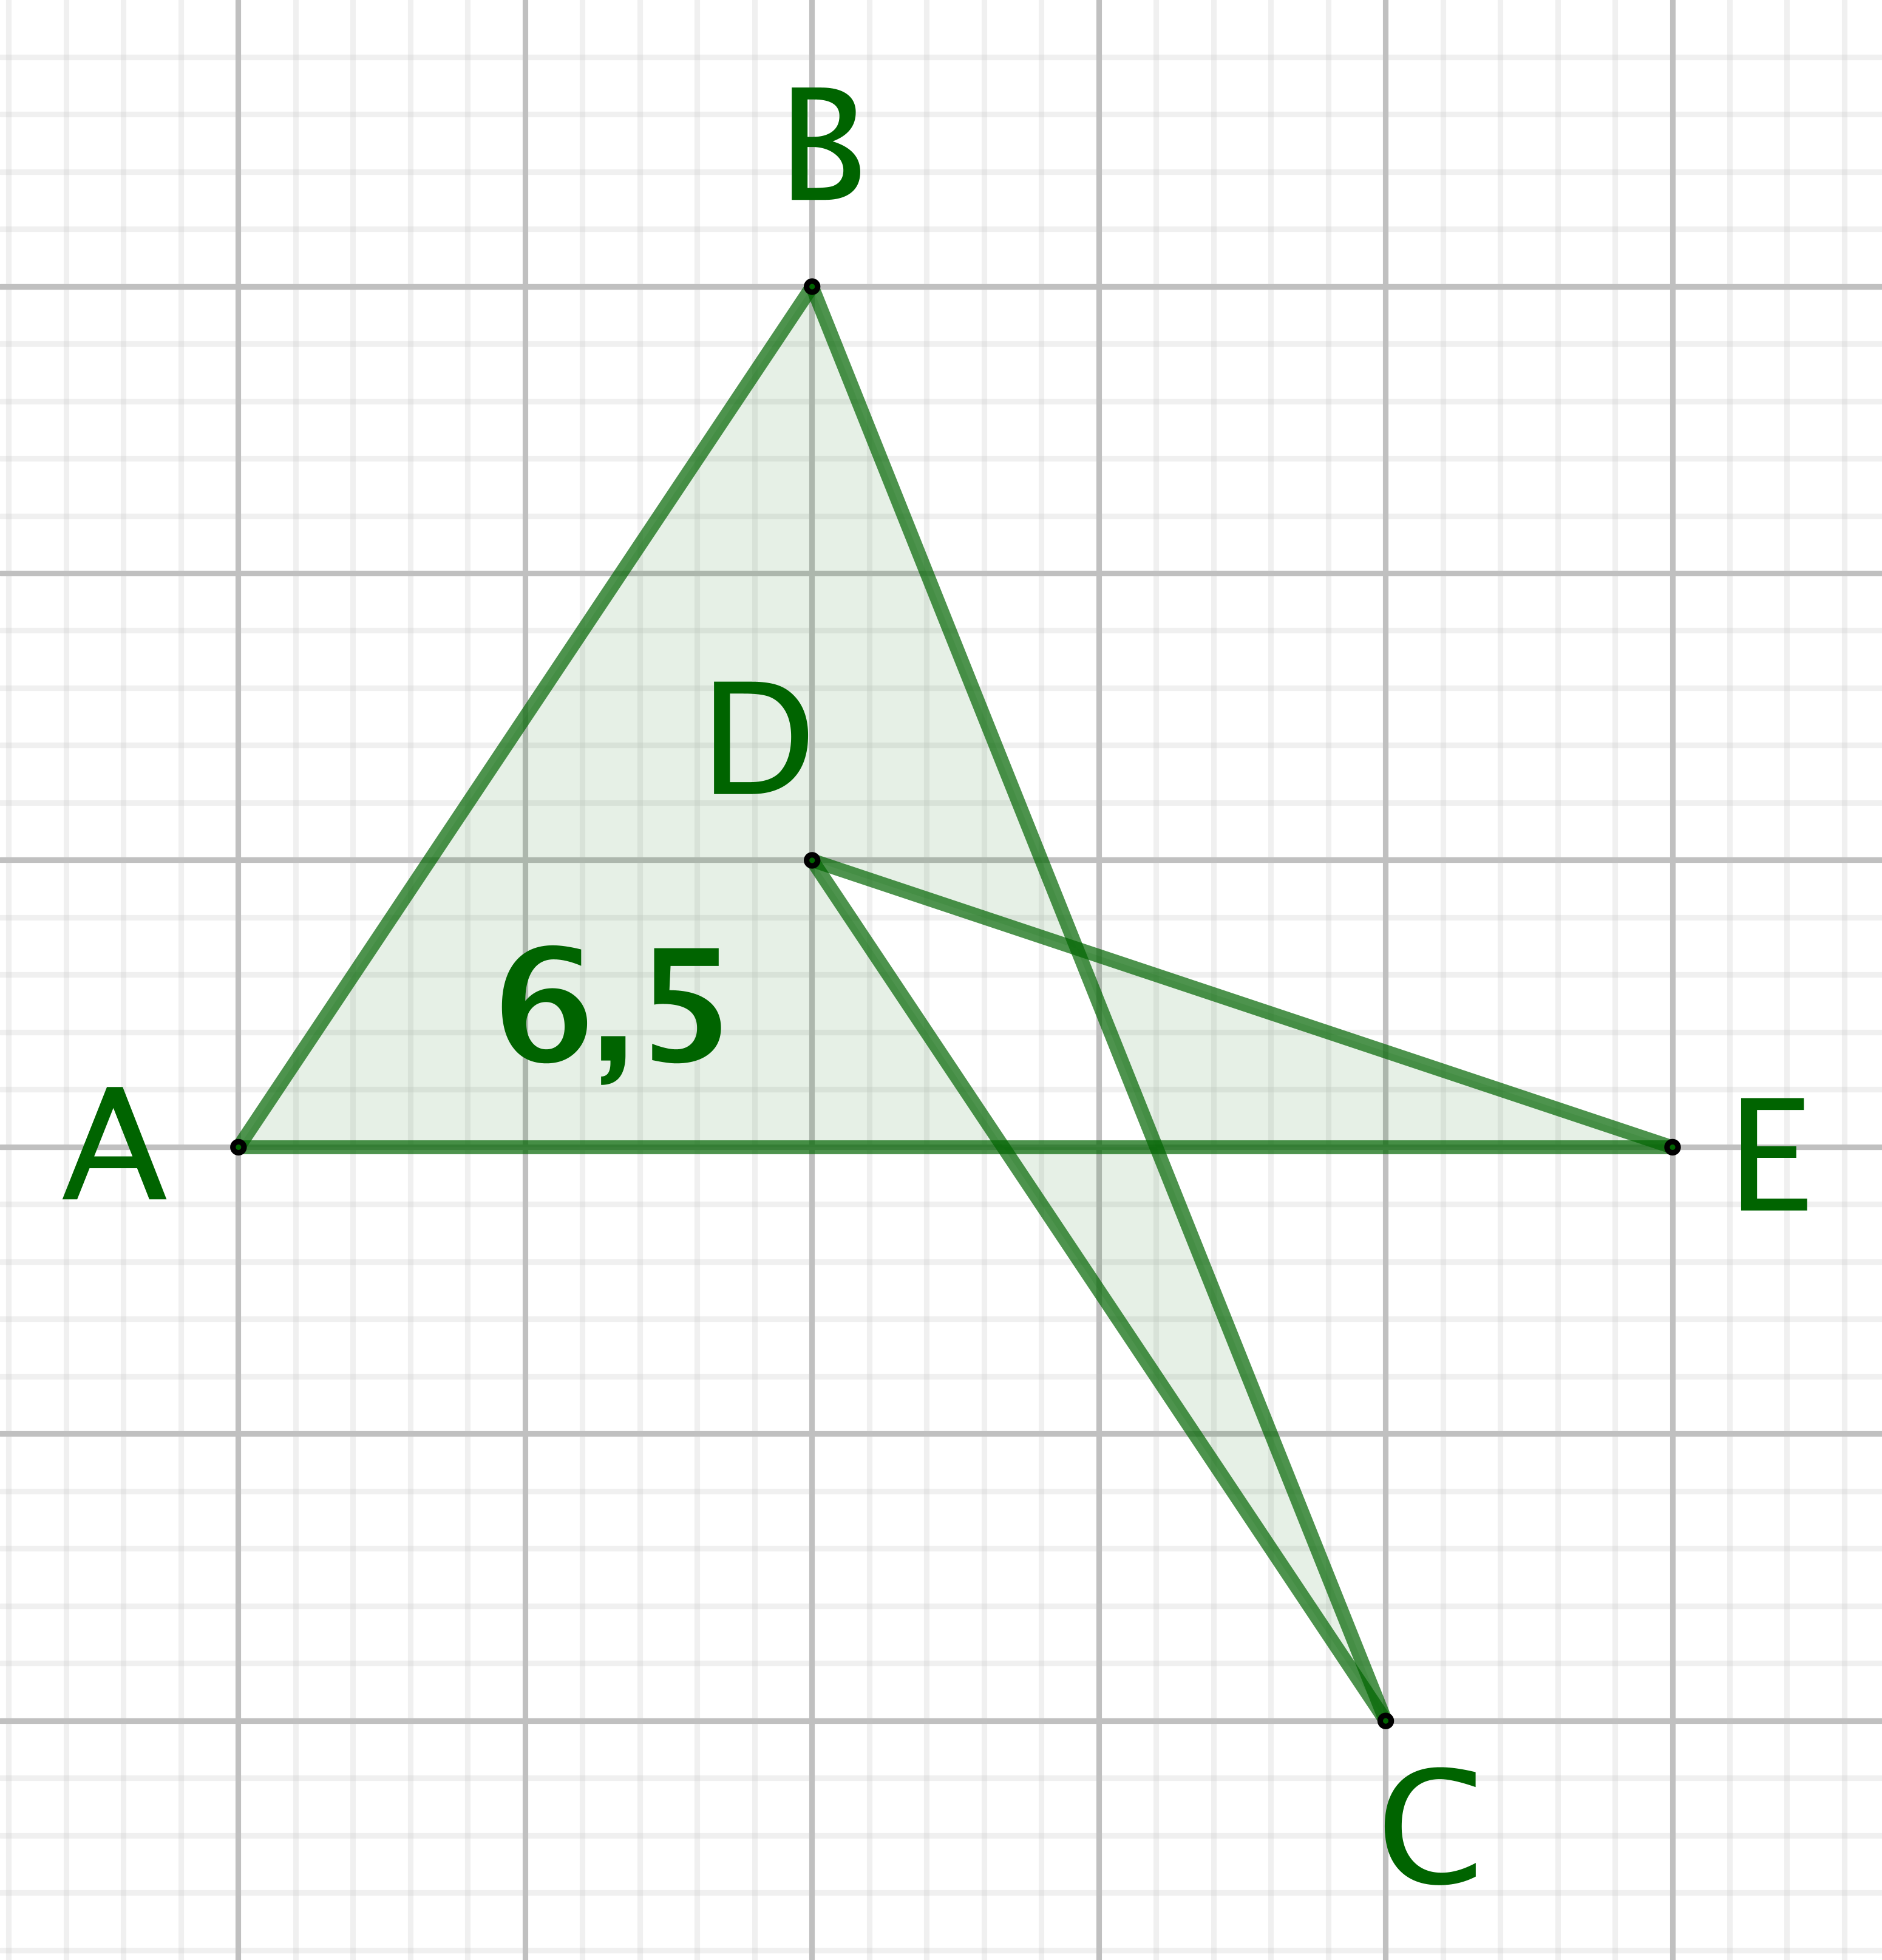
\includegraphics[scale=.4]{content/polygon/at-least-one/why.png}
    \end{center}

    \foreach \i in {3,1,4,2,5} {
    	\begin{center}
            \includegraphics[scale=.4]{content/polygon/at-least-one/why-step-\i.png}
        \end{center}
	}
\end{multicols}


Avant de formaliser ce qui précède, il faut noter que la notion d'aire algébrique est à manier avec prudence lorsqu'on la découvre.
Si c'est votre cas, que pensez-vous de l'aire algébrique du quadrilatère croisé $ABCD$ ci-dessous qui est un antiparallélogramme très particulier? Réponse en note de bas de page.%
\footnote{
    La réponse est $0$. Comme nous verrons que le choix de $\Omega$ est libre, il suffit de faire les calculs avec $\Omega$ l'intersection des segments $[AD]$ et $[BC]$.
    On peut donner du sens à ceci. Voici comment.
    Plongeons-nous dans l'espace.
    Imaginons une toile rectangulaire bleue sur le dessus, et rouge en dessous.
    Tournons de \qty{180}{\degree} verticalement l'un des côtés du rectangle.
    En supposant que la toile soit parfaitement tendue, nous obtenons, vue de dessus, un antiparallélogramme dont l'un des triangles est bleu, et l'autre rouge.
    De façon savante, les deux faces ont deux orientations différentes. Nous reparlerons de cette notion plus tard, c'est elle qui justifie les jeux de signes dans les calculs introductifs précédents.
}

\begin{center}
    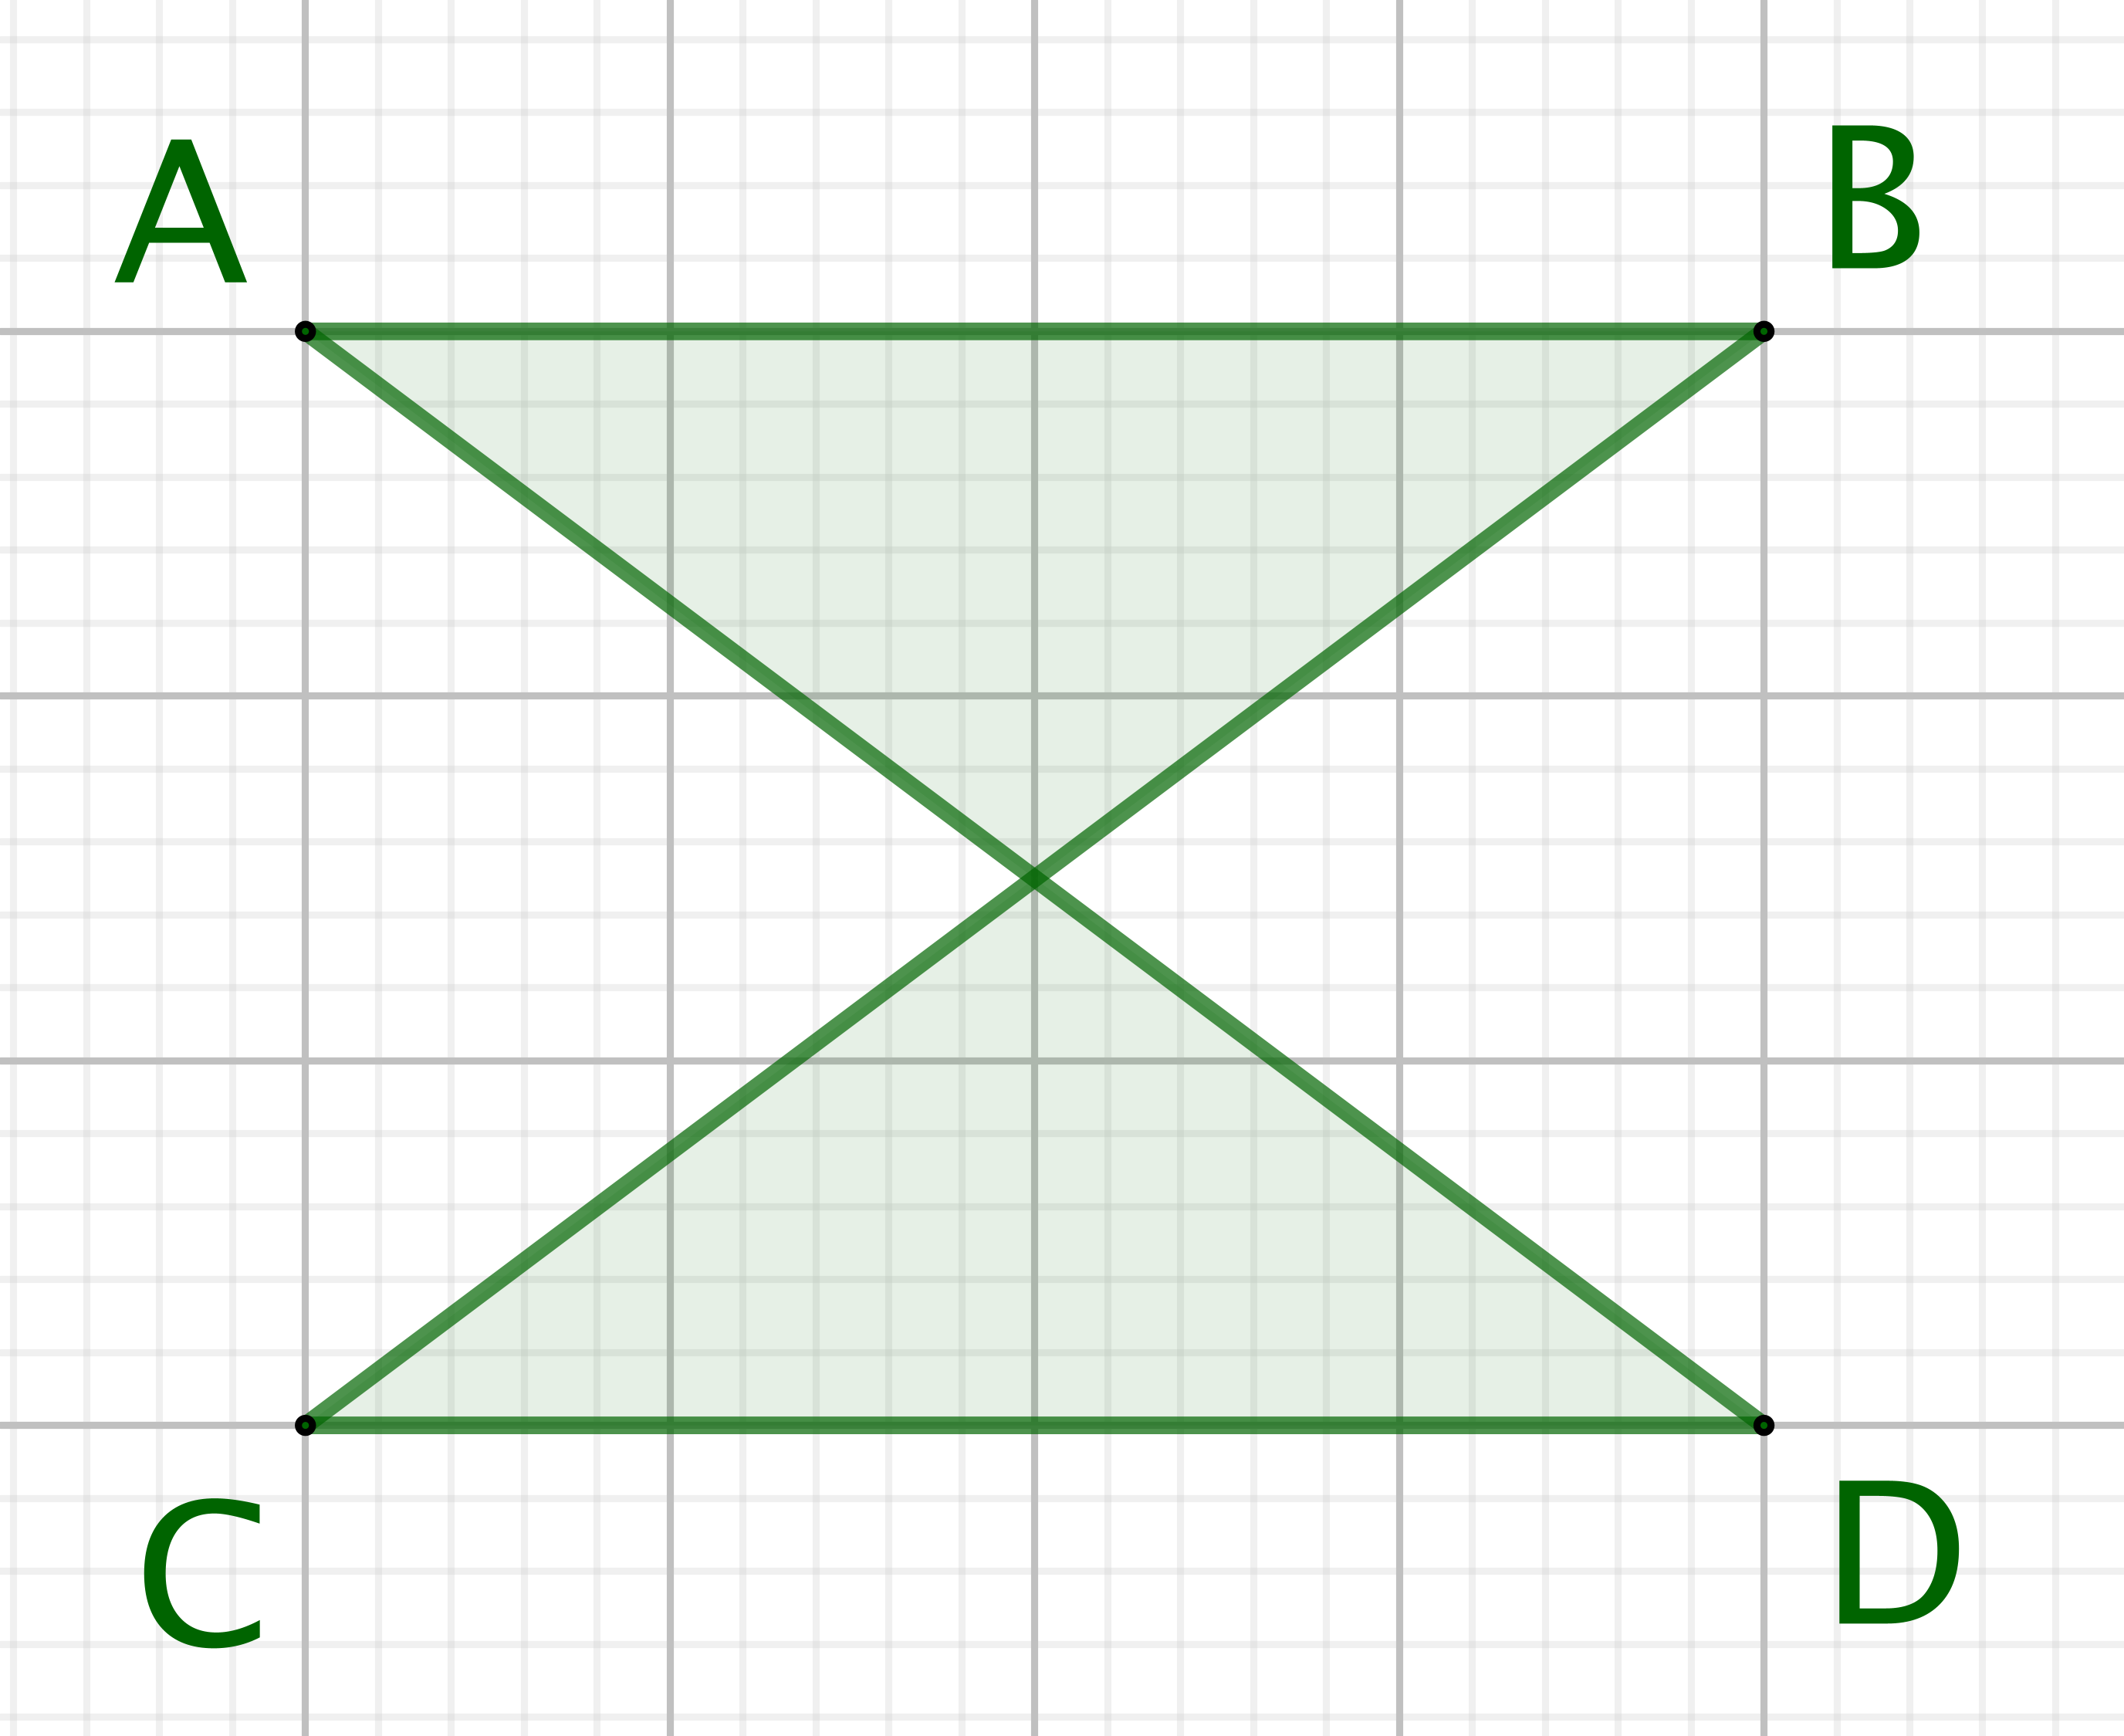
\includegraphics[scale=.4]{content/polygon/at-least-one/anti-para.png}
\end{center}


% ----------------------- %


\begin{defi} \label{garea-pt-ct}
    Pour tout \ncycle\ $\setproba{L} = A_1 A_2 \cdots A_n$, on définit $\big( A^{\,\prime}_i \big)_{i \in \ZZ}$ comme étant $n$-périodique, et vérifiant $A^{\,\prime}_{i} = A_i$ sur $\ZintervalC{1}{n}$.
\end{defi}


% ----------------------- %


\begin{fact} \label{garea-pt-ct}
    Soit $\setproba{L} = A_1 A_2 \cdots A_n$ un \ncycle.
    La fonction qui à un point $\Omega$ du plan associe
    $\mu_1^n (\Omega ;\setproba{L}) = \dsum_{i=1}^{n} \det \big( \vect{\Omega A^{\,\prime}_i} , \vect{\Omega A^{\,\prime}_{i+1}} \big)$ est indépendante du point $\Omega$.
    Dans la suite, cette quantité indépendante de $\Omega$ sera notée $\mu_1^n (\setproba{L})$.
\end{fact}


\begin{proof}
    Soit $M$ un autre point du plan.

    \begin{stepcalc}[style=ar*]
        \mu_1^n (\Omega ;\setproba{L})
    \explnext{}
        \dsum_{i=1}^{n} \det \big( \vect{\Omega A^{\,\prime}_i} , \vect{\Omega A^{\,\prime}_{i+1}} \big)
    \explnext*{Cette bonne vieille relation de Chasles.}{}
        \dsum_{i=1}^{n} \det \big( \vect{\Omega M} + \vect{M A^{\,\prime}_i} , \vect{\Omega M} + \vect{M A^{\,\prime}_{i+1}} \big)
    \explnext{}
        \dsum_{i=1}^{n} \Big[
            \det \big( \vect{\Omega M} , \vect{\Omega M} \big)
            +
            \det \big( \vect{\Omega M} , \vect{M A^{\,\prime}_{i+1}} \big)
            +
            \det \big( \vect{M A^{\,\prime}_i} , \vect{\Omega M} \big)
            +
            \det \big( \vect{M A^{\,\prime}_i} , \vect{M A^{\,\prime}_{i+1}} \big)
        \Big]
    \explnext{}
        \dsum_{i=1}^{n} \det \big( \vect{\Omega M} , \vect{M A^{\,\prime}_{i+1}} \big)
        +
        \dsum_{i=1}^{n} \det \big( \vect{M A^{\,\prime}_i} , \vect{\Omega M} \big)
        +
        \mu_1^n (M ; \setproba{L})
    \explnext{}
        \mu_1^n (M ; \setproba{L})
        +
        \dsum_{i=2}^{n+1} \det \big( \vect{\Omega M} , \vect{M A^{\,\prime}_{i}} \big)
        -
        \dsum_{i=1}^{n} \det \big( \vect{\Omega M} , \vect{M A^{\,\prime}_i} \big)
    \explnext{}
        \mu_1^n (M ; \setproba{L})
        +
        \det \big( \vect{\Omega M} , \vect{M A^{\,\prime}_{n+1}} \big)
        -
        \det \big( \vect{\Omega M} , \vect{M A^{\,\prime}_1} \big)
    \explnext*{$A^{\,\prime}_{n+1} = A^{\,\prime}_1$}{}
        \mu_1^n (M ; \setproba{L})
    \end{stepcalc}

    \null\vspace{-3.5ex}
\end{proof}


% ----------------------- %


\begin{fact} \label{nline-shift-inva}
    Soit $\setproba{L} = A_1 A_2 \cdots A_n$ un \ncycle.
    Pour $k \in \ZintervalC{1}{n}$,
    le \ncycle\ $\setproba{L}_j = B_1 B_2 \cdots B_n$, où $B_i = A^{\,\prime}_{i+k-1}$,
    vérifie
    $\mu_1^n (\setproba{L}) = \mu_1^n (\setproba{L}_k)$.
    Dans la suite, cette quantité commune sera notée $\mu (\setproba{L})$.
\end{fact}


\begin{proof}
    Il suffit de s'adonner à un petit jeu sur les indices de sommation.
\end{proof}


% ----------------------- %


\begin{fact} \label{nline-rota-inva}
    Soit
    $\setproba{L} = A_1 A_2 \cdots A_n$ un \ncycle.
    le \ncycle\ $\setproba{L}^{\mathrm{op}} = B_1 B_2 \cdots B_n$, où $B_i =  A_{n + 1 - i}$,
    vérifie
    $\mu(\setproba{L}^{\mathrm{op}}) = {} - \mu(\setproba{L})$.
\end{fact}


\begin{proof}
    Soit $\Omega$ un point quelconque du plan.

    \begin{stepcalc}[style=ar*]
        \mu(\setproba{L}^{\mathrm{op}})
    \explnext{}
        \dsum_{i=1}^{n} \det \big( \vect{\Omega B^{\,\prime}_i} , \vect{\Omega B^{\,\prime}_{i+1}} \big)
    \explnext{}
        \dsum_{i=1}^{n} \det \big( \vect{\Omega A^{\,\prime}_{n + 1 - i}} , \vect{\Omega A^{\,\prime}_{n - i}} \big)
    \explnext{}
        \dsum_{j=0}^{n-1} \det \big( \vect{\Omega A^{\,\prime}_{j + 1}} , \vect{\Omega A^{\,\prime}_j} \big)
    \explnext*{$A^{\,\prime}_0 = A^{\,\prime}_n$ et $A^{\,\prime}_1 = A^{\,\prime}_{n+1}$}{}
        \dsum_{j=1}^{n} \det \big( \vect{\Omega A^{\,\prime}_{j + 1}} , \vect{\Omega A^{\,\prime}_j} \big)
    \explnext{}
        {} - \dsum_{j=1}^{n} \det \big( \vect{\Omega A^{\,\prime}_j} ,  \vect{\Omega A^{\,\prime}_{j + 1}} \big)
    \explnext{}
        {} - \mu(\setproba{L})
    \end{stepcalc}

    \null\vspace{-3.5ex}
\end{proof}


% ----------------------- %


\begin{fact}
    Soit
    $\setproba{L} = A_1 A_2 \cdots A_n$ un \ncycle.
    La quantité $\frac12 \abs{\mu(\setproba{L})}$ ne dépend ni du sens de parcours de $\setproba{L}$, ni du point de départ choisi.%
    \footnote{
        Le lecteur pardonnera les abus de langage utilisés.
    }
    Elle sera notée $\garea{\setproba{L}}$, 
    et nommée \og \emph{aire généralisée} \fg\ du \ncycle\ $\setproba{L}$, 
    tandis que $\frac12 \mu(\setproba{L})$ 
    sera appelé \og \emph{aire algébrique} \fg\ de $\setproba{L}$.
\end{fact}


\begin{proof}
    C'est une conséquence directe des faits \ref{nline-shift-inva} et \ref{nline-rota-inva}.
\end{proof}


% ----------------------- %


Dans la suite, nous aurons besoin de savoir que 
$\garea{\setproba{P}} = \area{\setproba{P}}$ pour tout \ngone\ $\setproba{P}$.%
%\footnote{
%	Nous obtenons ainsi la généralisation de l'aire géométrique usuelle au cas des polygones croisés.
%}
Ceci est évident dans le cas convexe, car il suffit de choisir l'isobarycentre $G$ de $A_1$, $A_2$, ..., $A_n$ pour le calcul de $\garea{\setproba{P}}$: en effet, avec ce choix, tous les déterminants $\det \big( \vect{G A^{\,\prime}_i} , \vect{G A^{\,\prime}_{i+1}} \big)$ ont le même signe.
Dans le cas non-convexe, les choses se compliquent a priori, car nous ne maîtrisons plus les signes des déterminants. Heureusement, nous avons le résultat suivant.


\begin{fact} \label{route-direction}
    Soit un \ngone\ $\setproba{P}$ de \ncycle\ associé $\setproba{L} = A_1 A_2 \cdots A_n$ tel que $A_1$, $A_2$, ..., $A_n$ soient parcourus dans le sens trigonométrique, ou anti-horaire.
    Un tel \ncycle\ sera dit \og \emph{positif} \fg.%
    \footnote{
    	Bien noté que cette notion ne peut pas exister pour un polygone croisé. De façon cachée, nous utilisons le célèbre théorème de Jordan, dans sa forme polygonale.
    }
    Sous cette hypothèse, nous avons $\mu(\setproba{L}) \geq 0$.
\end{fact}


\begin{proof}
	Le théorème de triangulation affirme que tout \ngone\ est triangulable comme dans l'exemple très basique suivant qui laisse envisager une démonstration par récurrence en retirant l'un des triangles ayant deux côtés correspondant à deux côtés consécutifs du \ngone\ (pour peu qu'un tel triangle existe toujours).


    \begin{multicols}{3}
        \small\itshape
        \begin{center}
            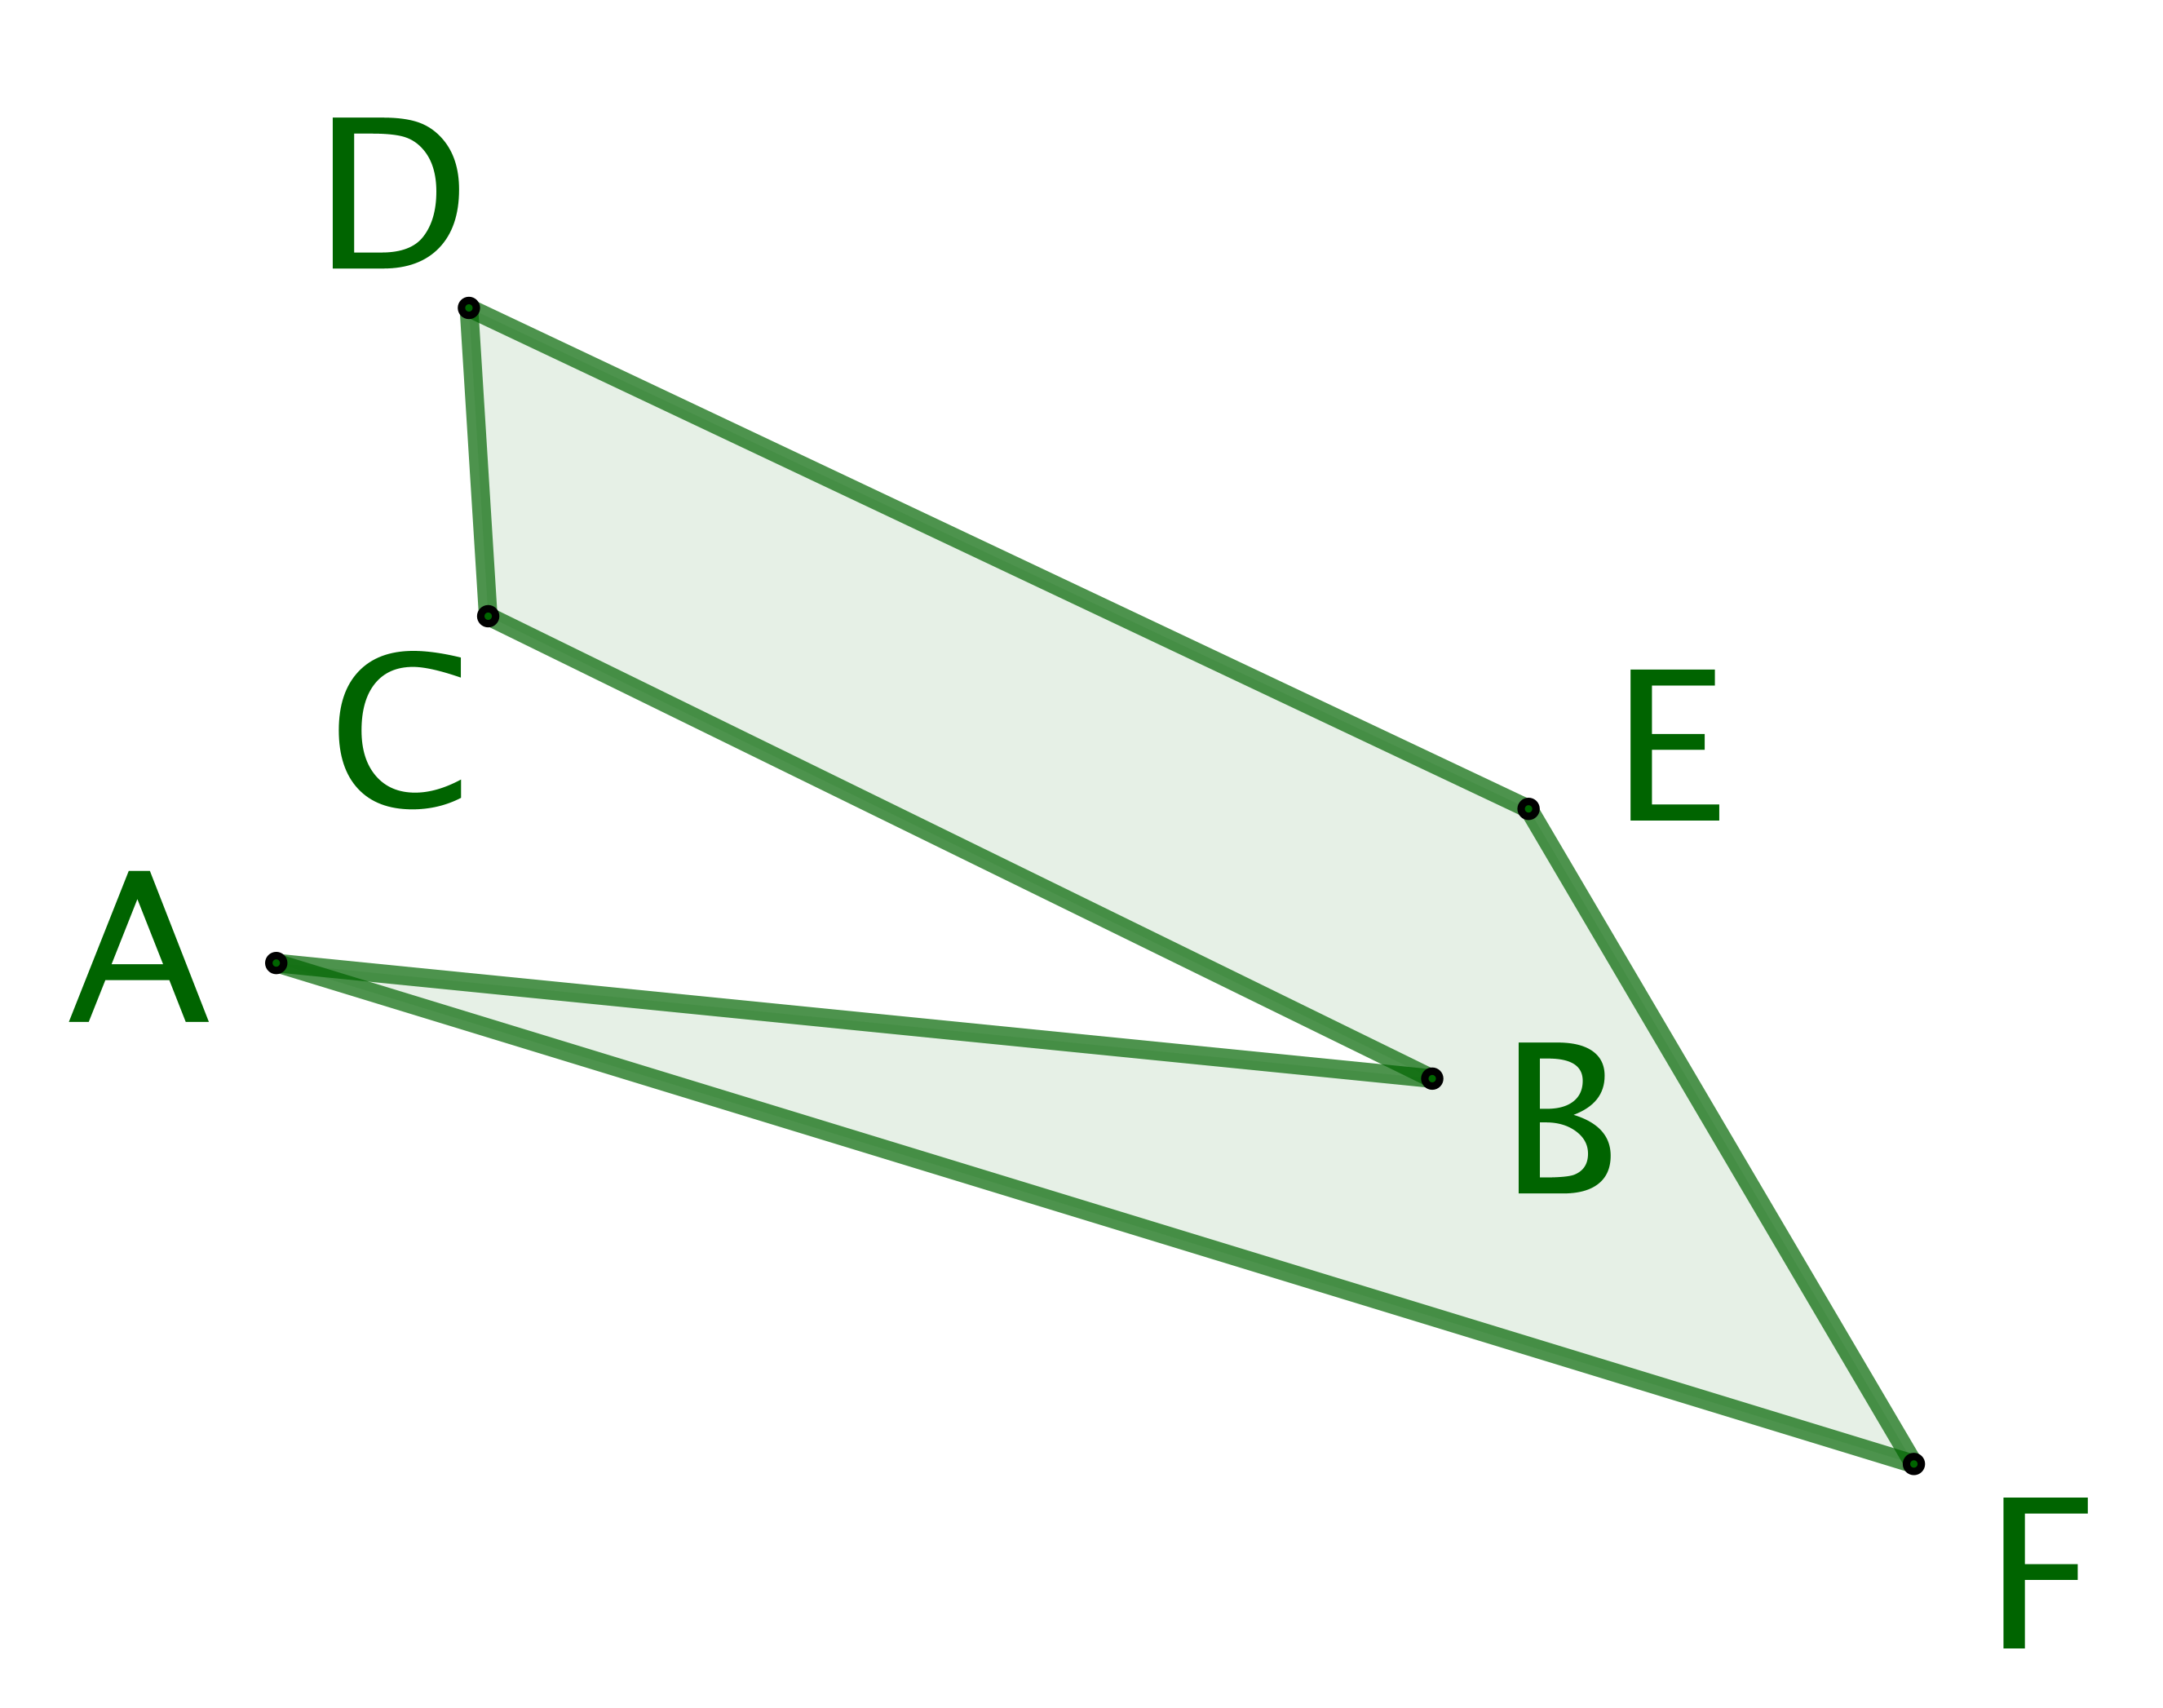
\includegraphics[scale=.4]{content/polygon/at-least-one/triangulation-1.png}

            \smallskip
            Un \ngone\ \og nu \fg.
        \end{center}


        \begin{center}
            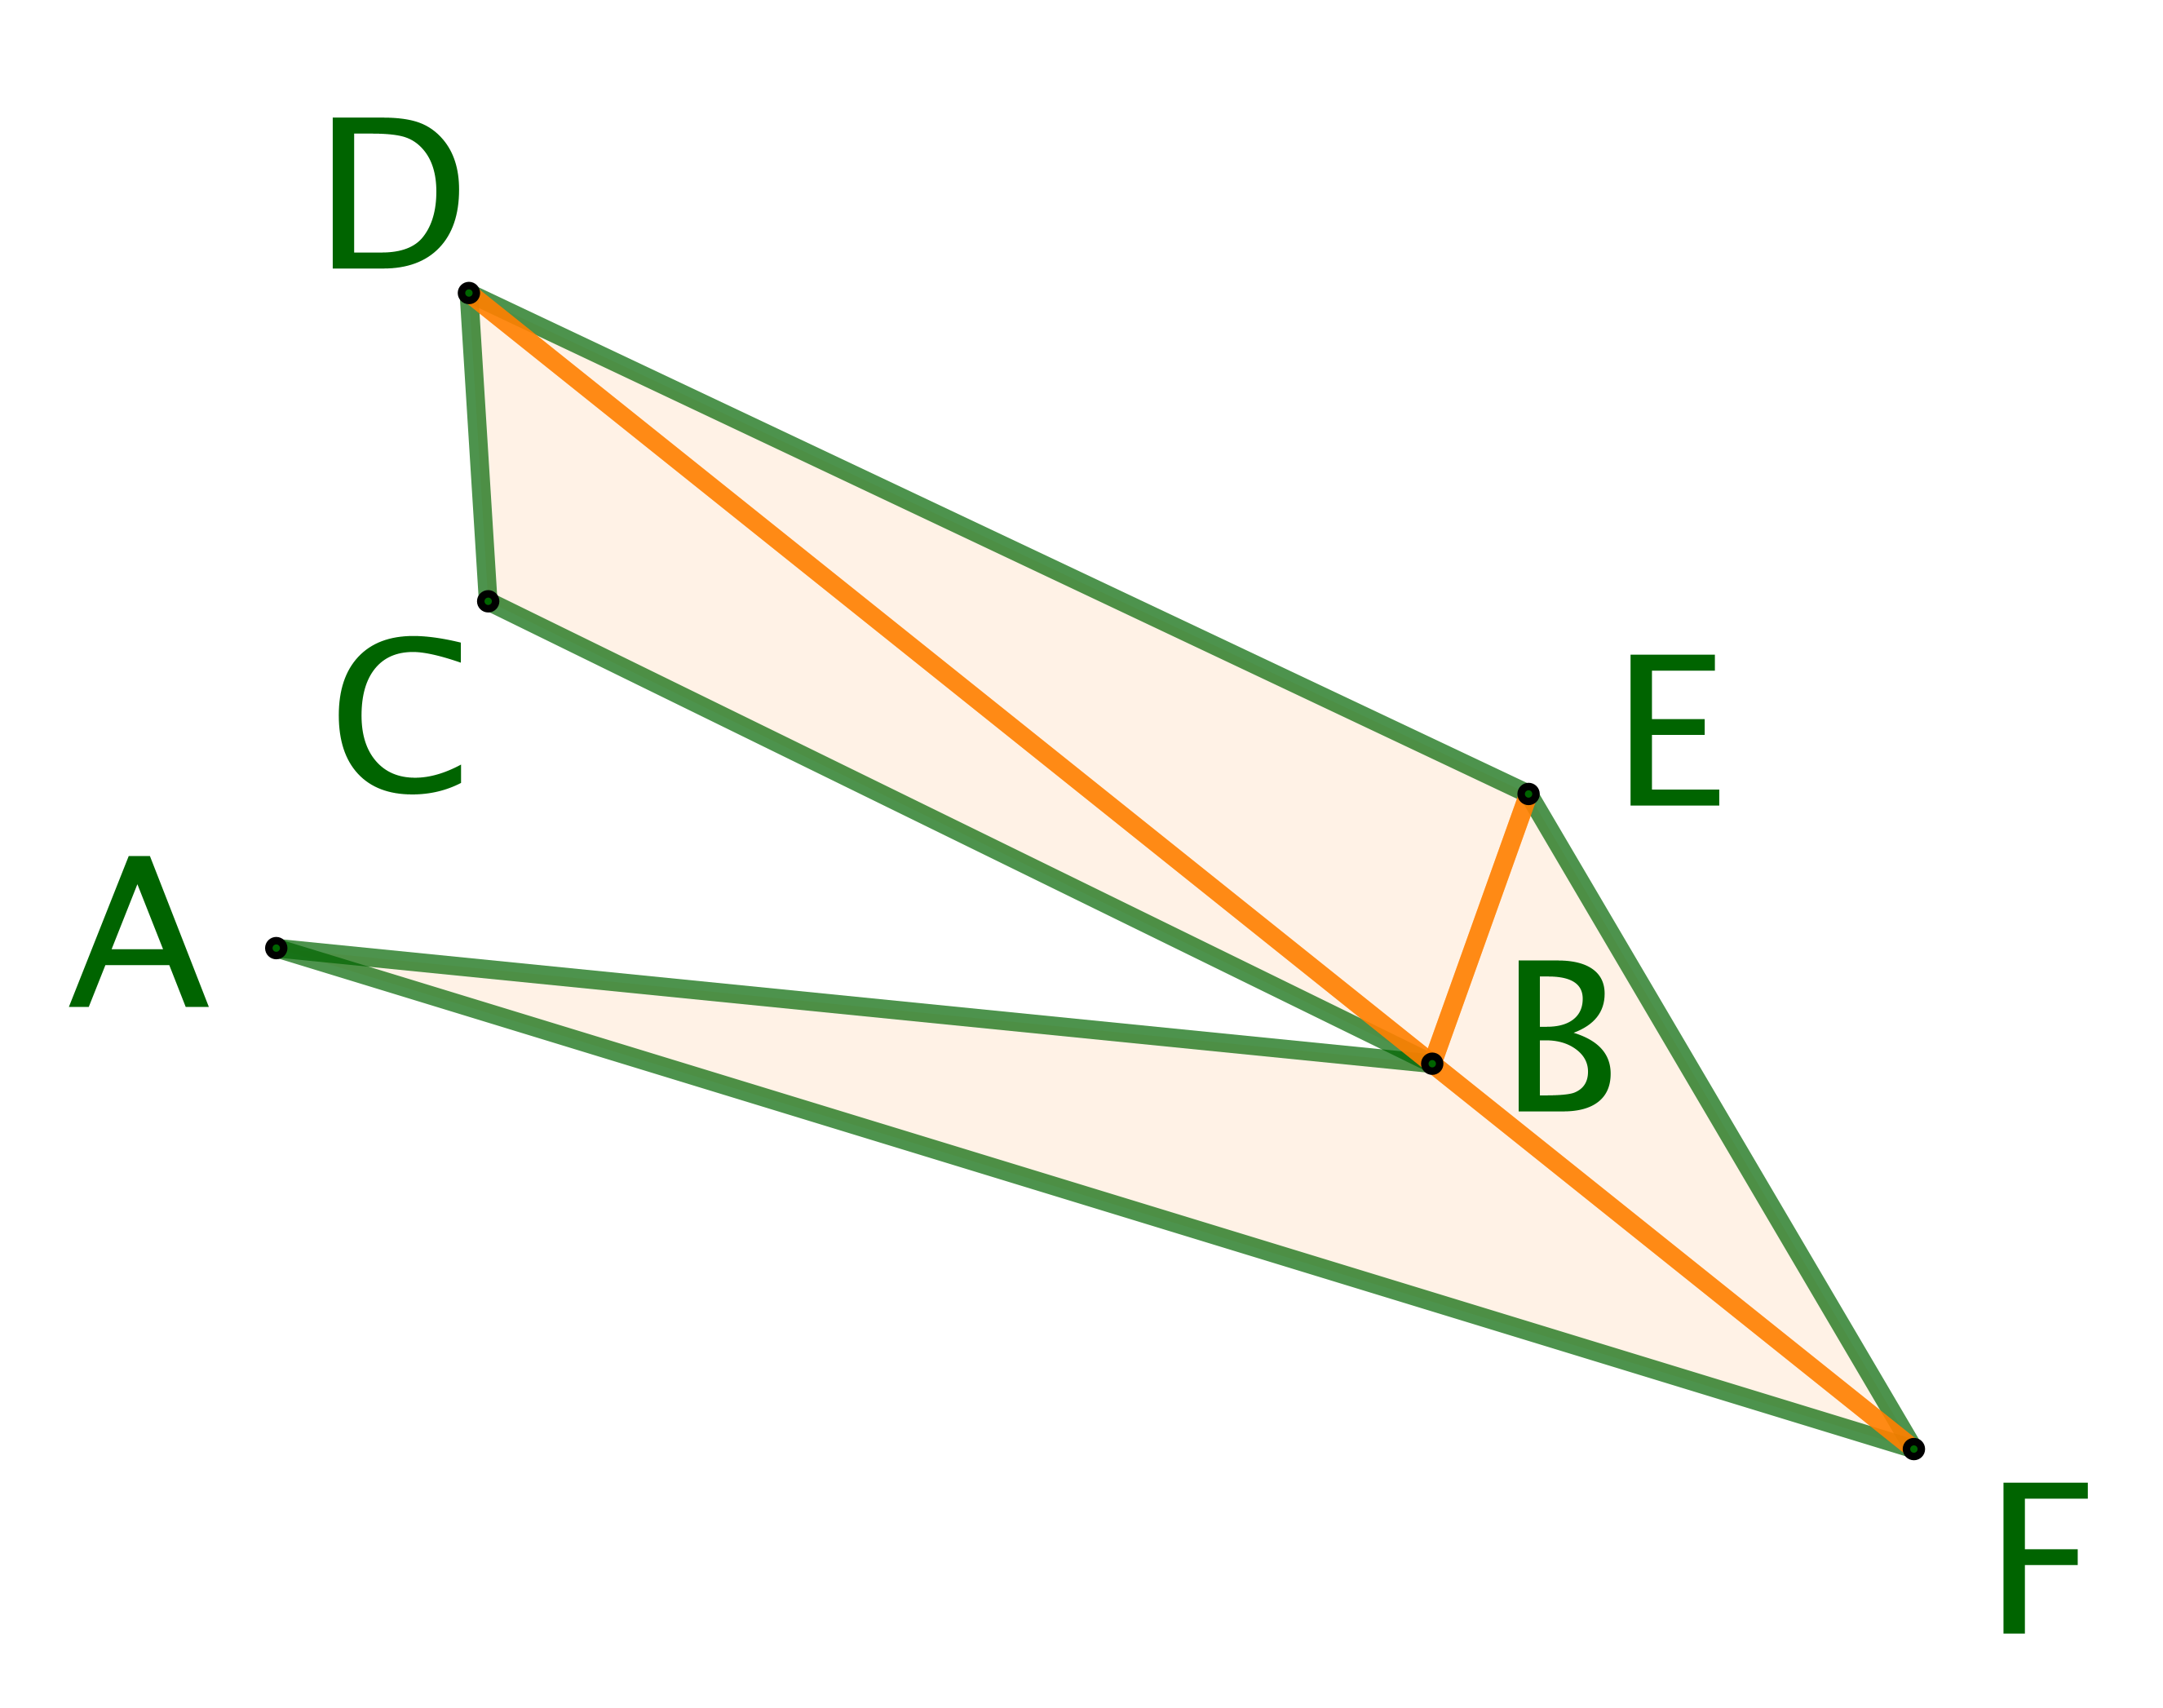
\includegraphics[scale=.4]{content/polygon/at-least-one/triangulation-2.png}

            \smallskip
            Le \ngone\ triangulé.
        \end{center}


        \begin{center}
            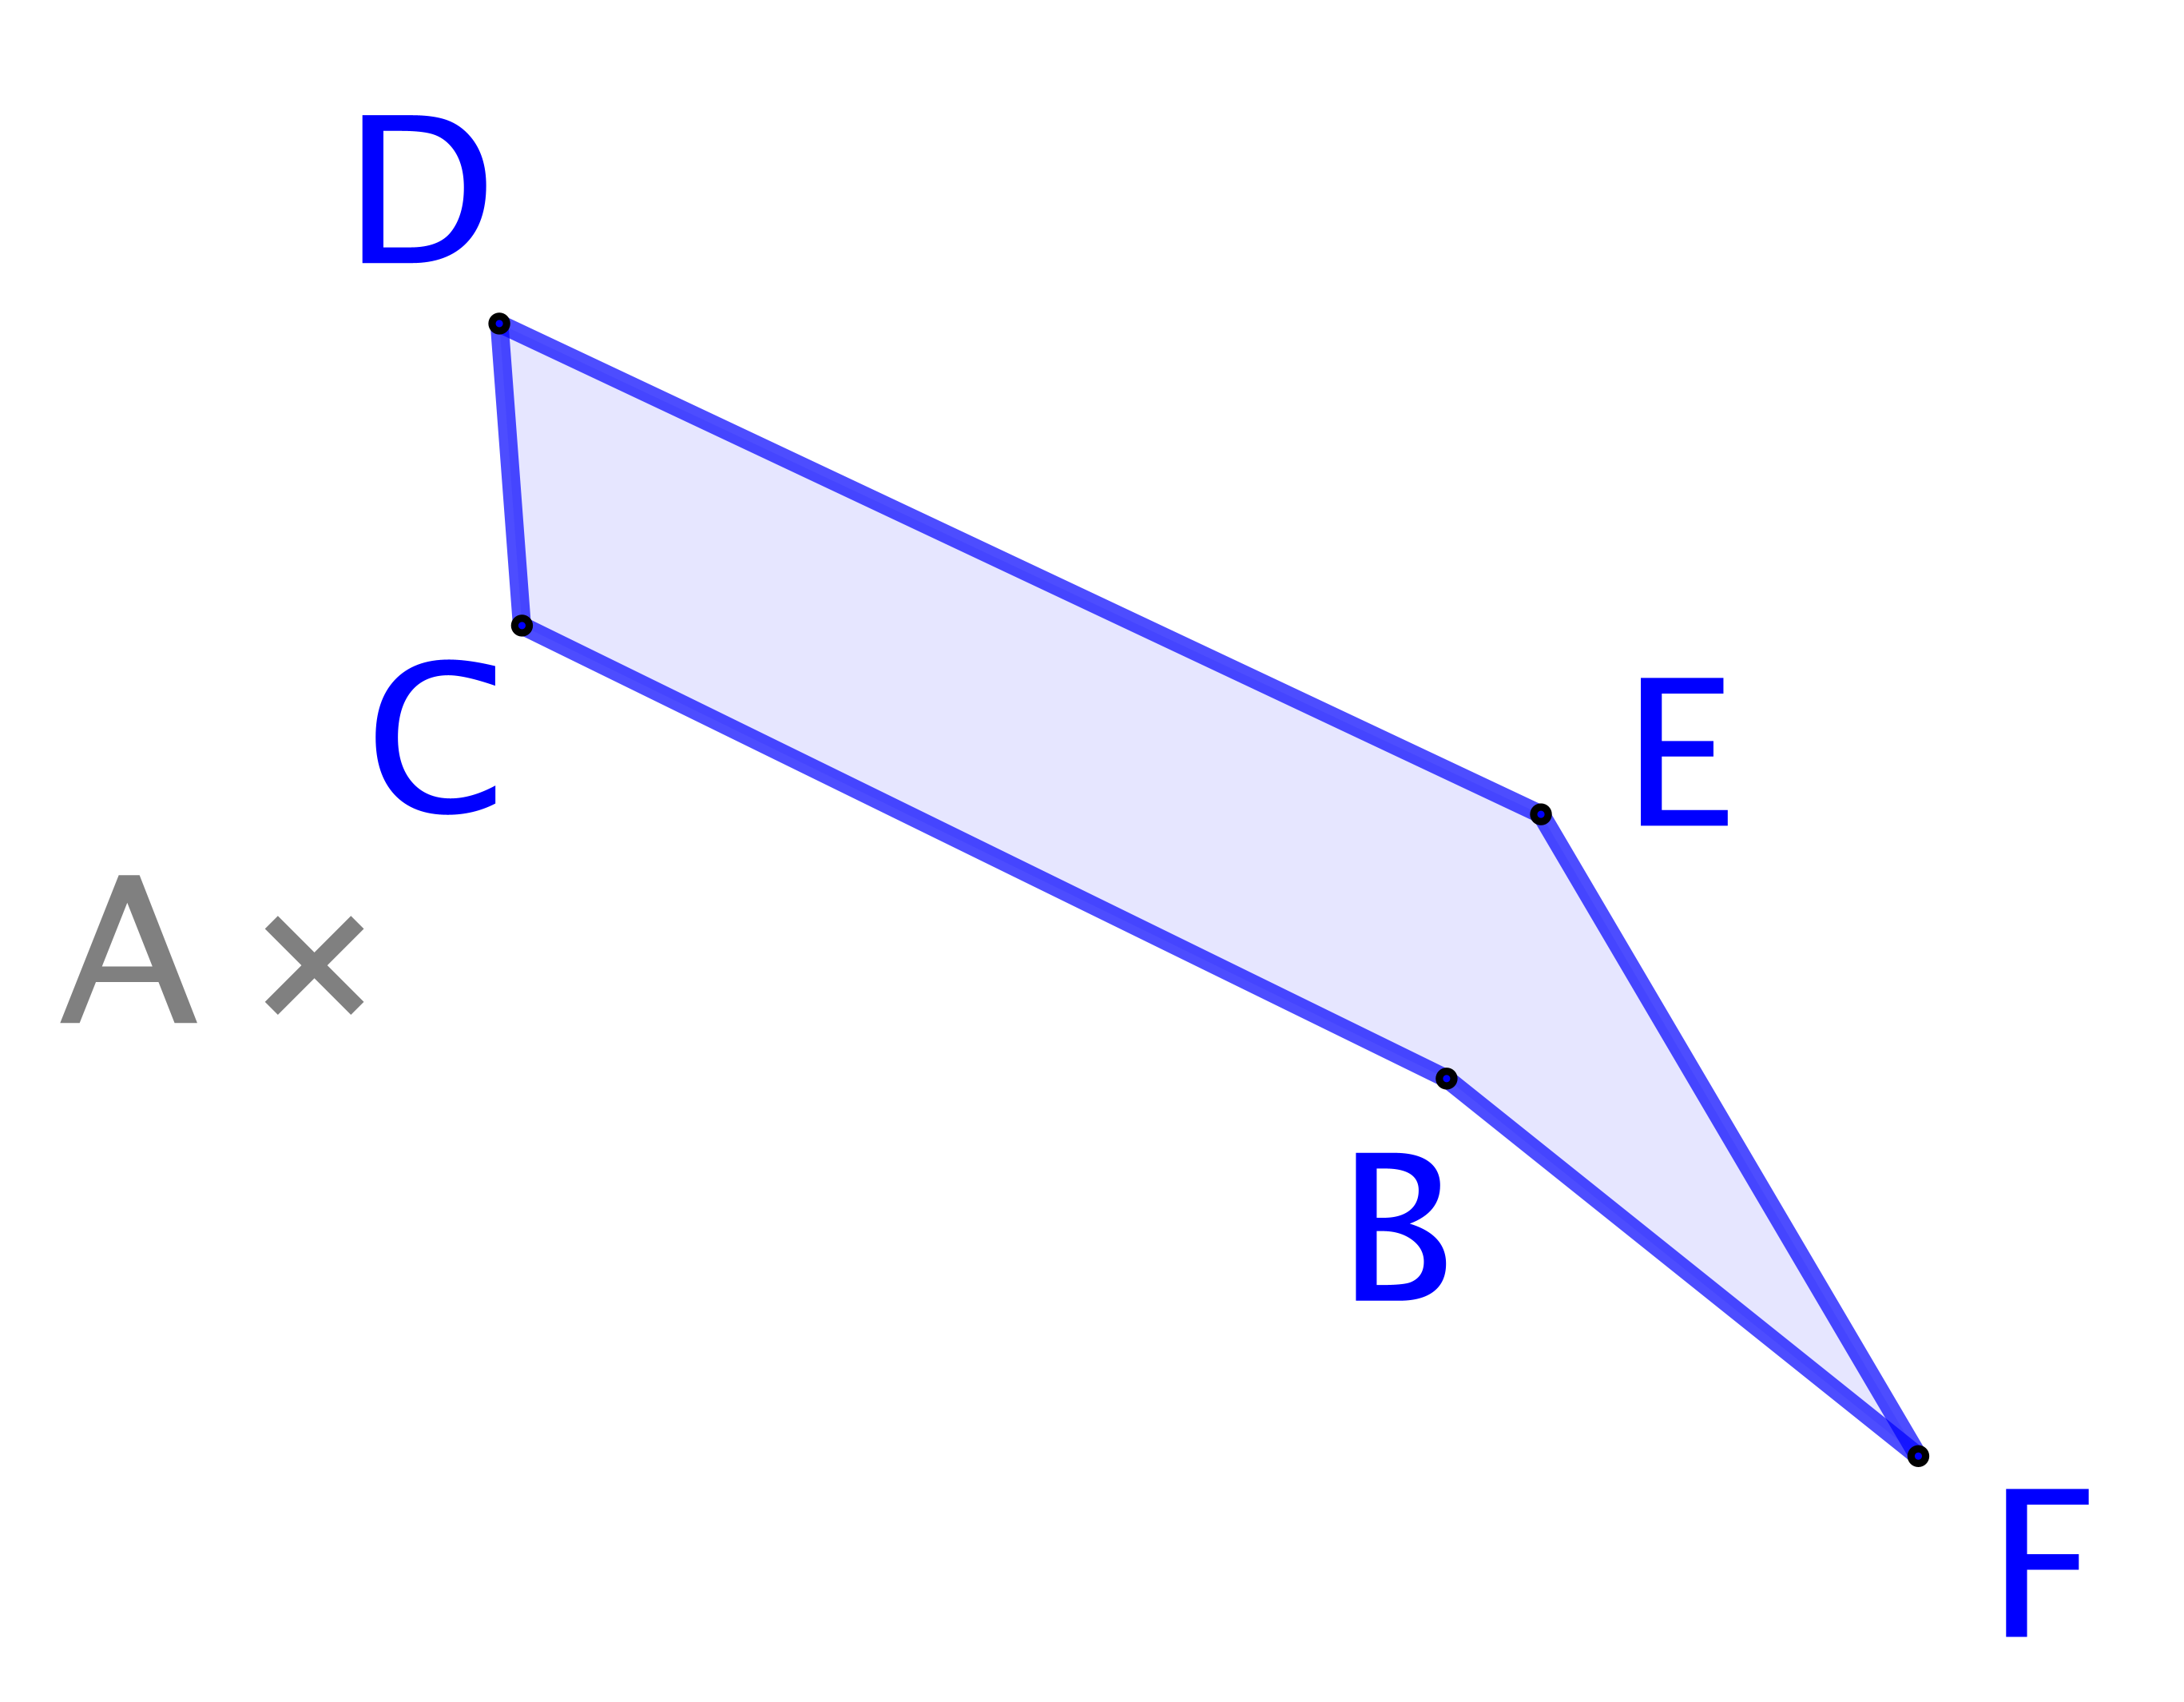
\includegraphics[scale=.4]{content/polygon/at-least-one/triangulation-3.png}

            \smallskip
            Le \ngone\ allégé.
        \end{center}
    \end{multicols}


    Le théorème de triangulation admet une forme forte donnant une décomposition contenant un triangle formé de deux côtés consécutifs du \ngone.%
    \footnote{
        En pratique, cette forme forte est peu utile, car elle aboutit à un algorithme de recherche trop lent.
    }
    Nous dirons qu'une telle décomposition est \og \emph{à l'écoute} \fg.
    Ce très mauvais jeu de mots fait référence à la notion sérieuse \og \emph{d'oreille} \fg\ pour un \ngone: une oreille est un triangle inclus dans le \ngone, et formé de deux côtés consécutifs du \ngone.
    L'exemple suivant donne un \ngone\ ayant juste deux oreilles.%
    \footnote{
        On démontre que tout \ngone\ admet au minimum deux oreilles.
    }


    \begin{multicols}{2}
        \small\itshape
    	\begin{center}
        	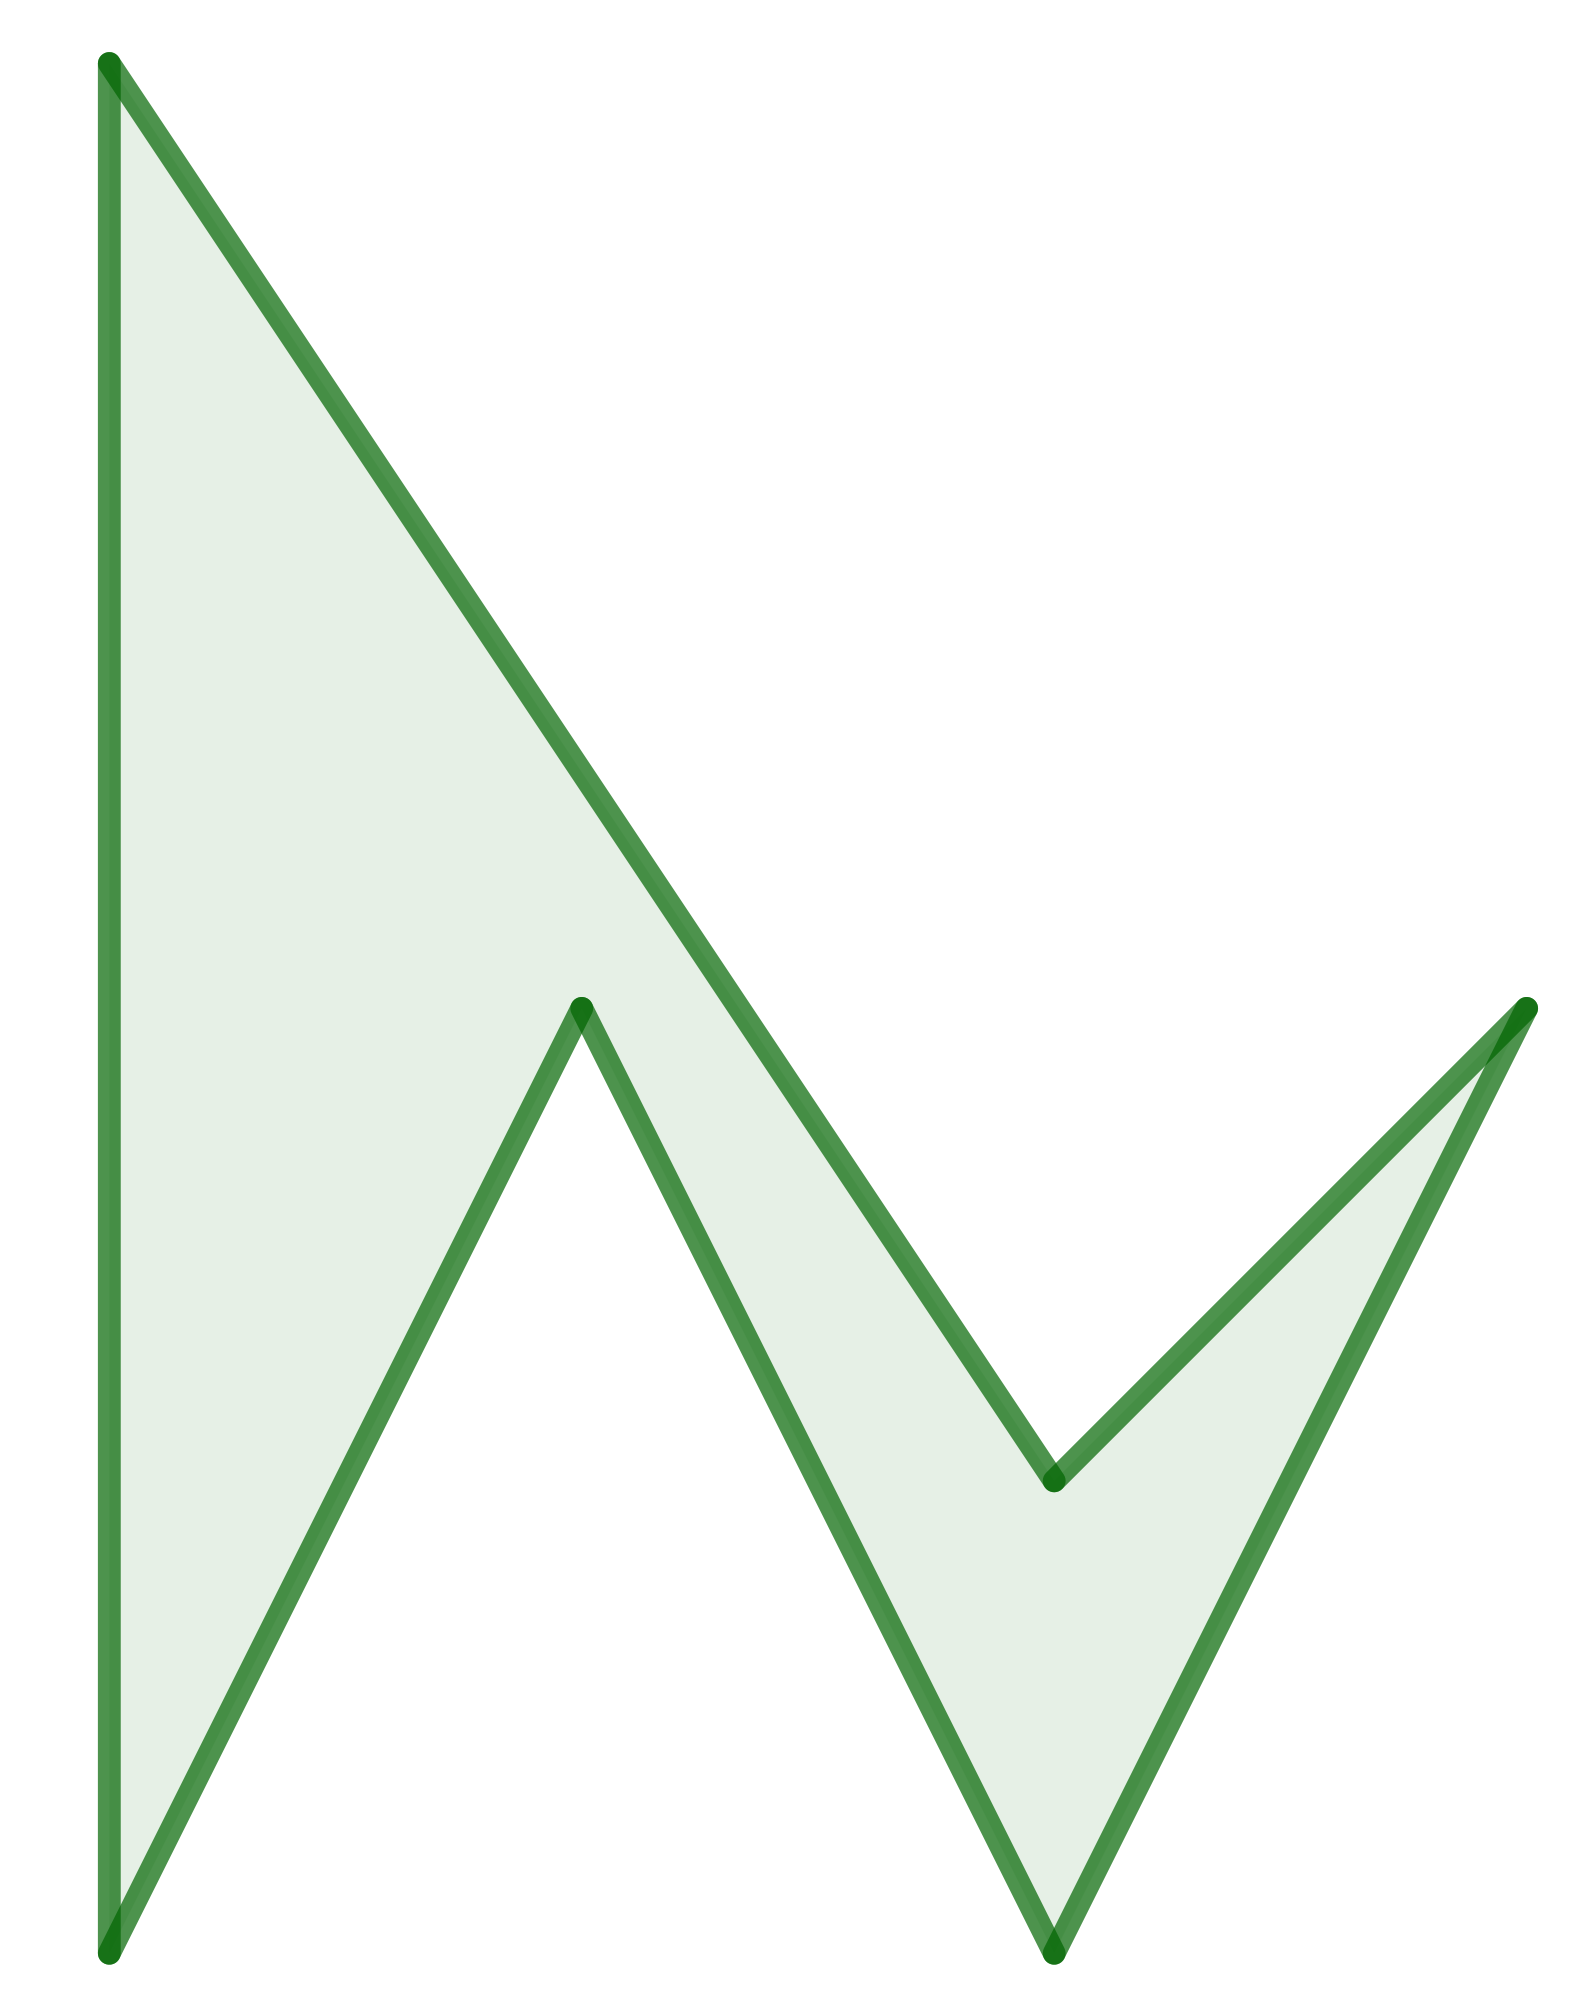
\includegraphics[scale=.4]{content/polygon/at-least-one/mini-ear-1.png}

        	\smallskip
       		Un \ngone\ basique.
    	\end{center}

    	\begin{center}
        	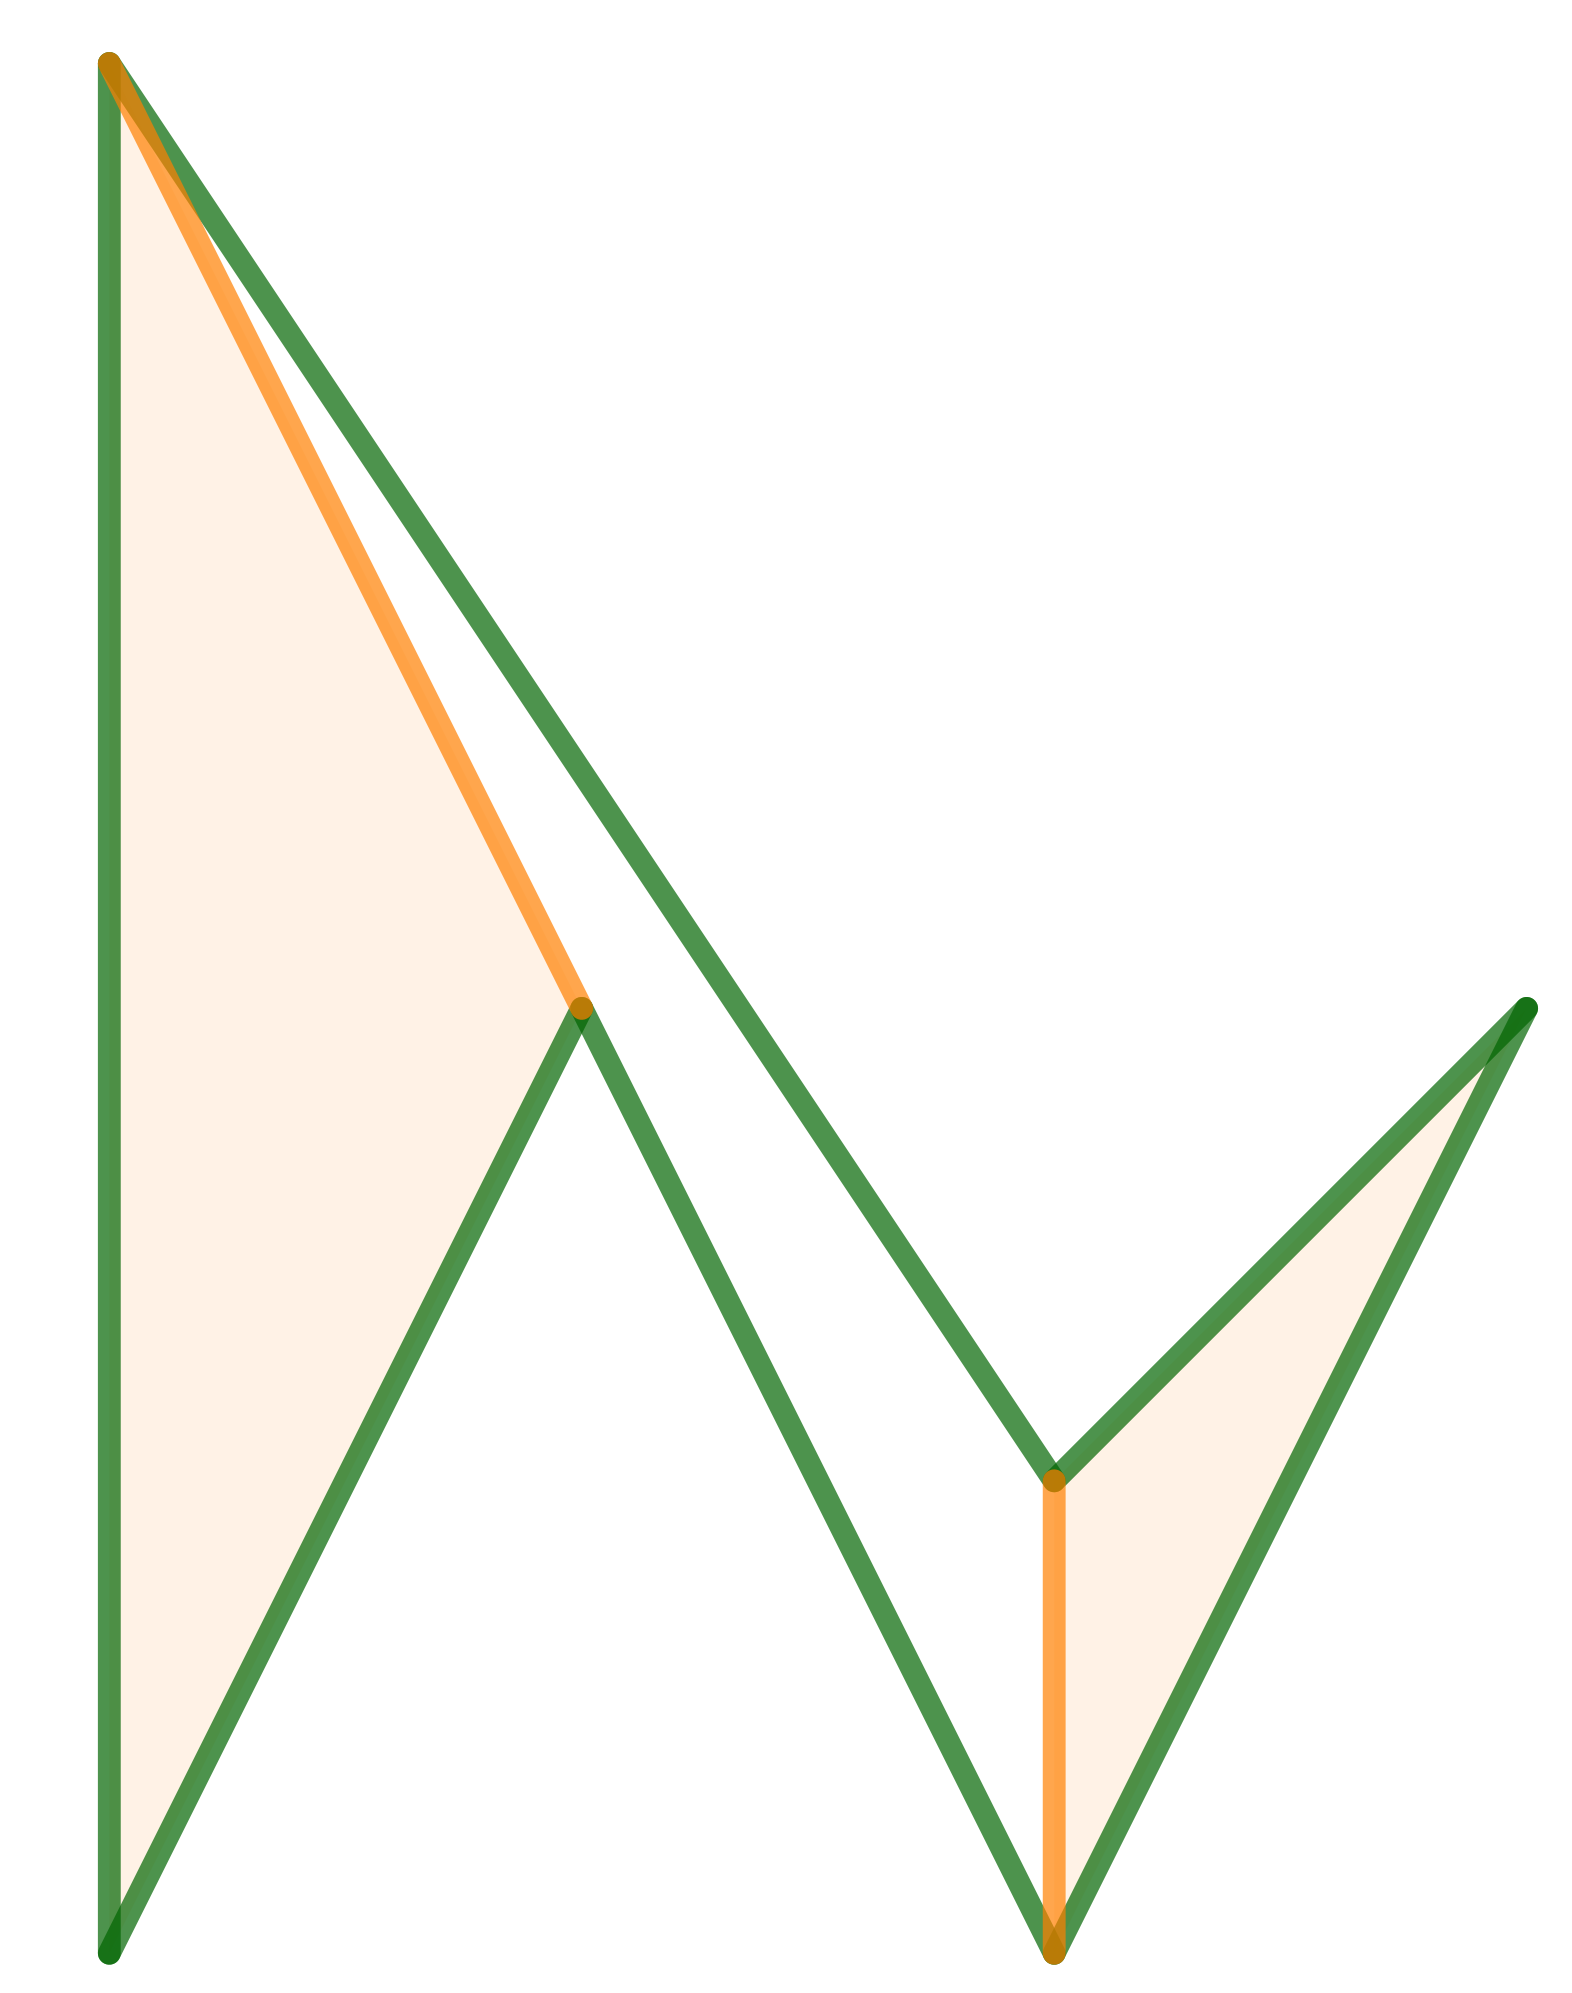
\includegraphics[scale=.4]{content/polygon/at-least-one/mini-ear-2.png}

        	\smallskip
       		Juste deux oreilles disponibles.
    	\end{center}
    \end{multicols}


	Raisonnons donc par récurrence sur $n \in \NN_{\geq3}$.

	\begin{itemize}
		\item \textbf{Cas de base.}
		Soit $ABC$ un triangle. Dire que les sommets $A$, $B$ et $C$ sont parcourus dans le sens trigonométrique, c'est savoir que $\mu(ABC) = \det \big( \vect{AB} , \vect{AC} \big) > 0$.


		\item \textbf{Hérédité.}
		Soient un \ngone\ $\setproba{P}$, avec $n \in \NN_{>3}$, et $\setproba{L} = A_1 A_2 \cdots A_n$ un \ncycle\ positif qui lui est associée. On peut supposer que $A_{n-1} A_n A_1$ est une oreille d'une triangulation à l'écoute du \ngone\ $\setproba{P}$.


	    \begin{multicols}{2}
    	    \small\itshape
    		\begin{center}
        	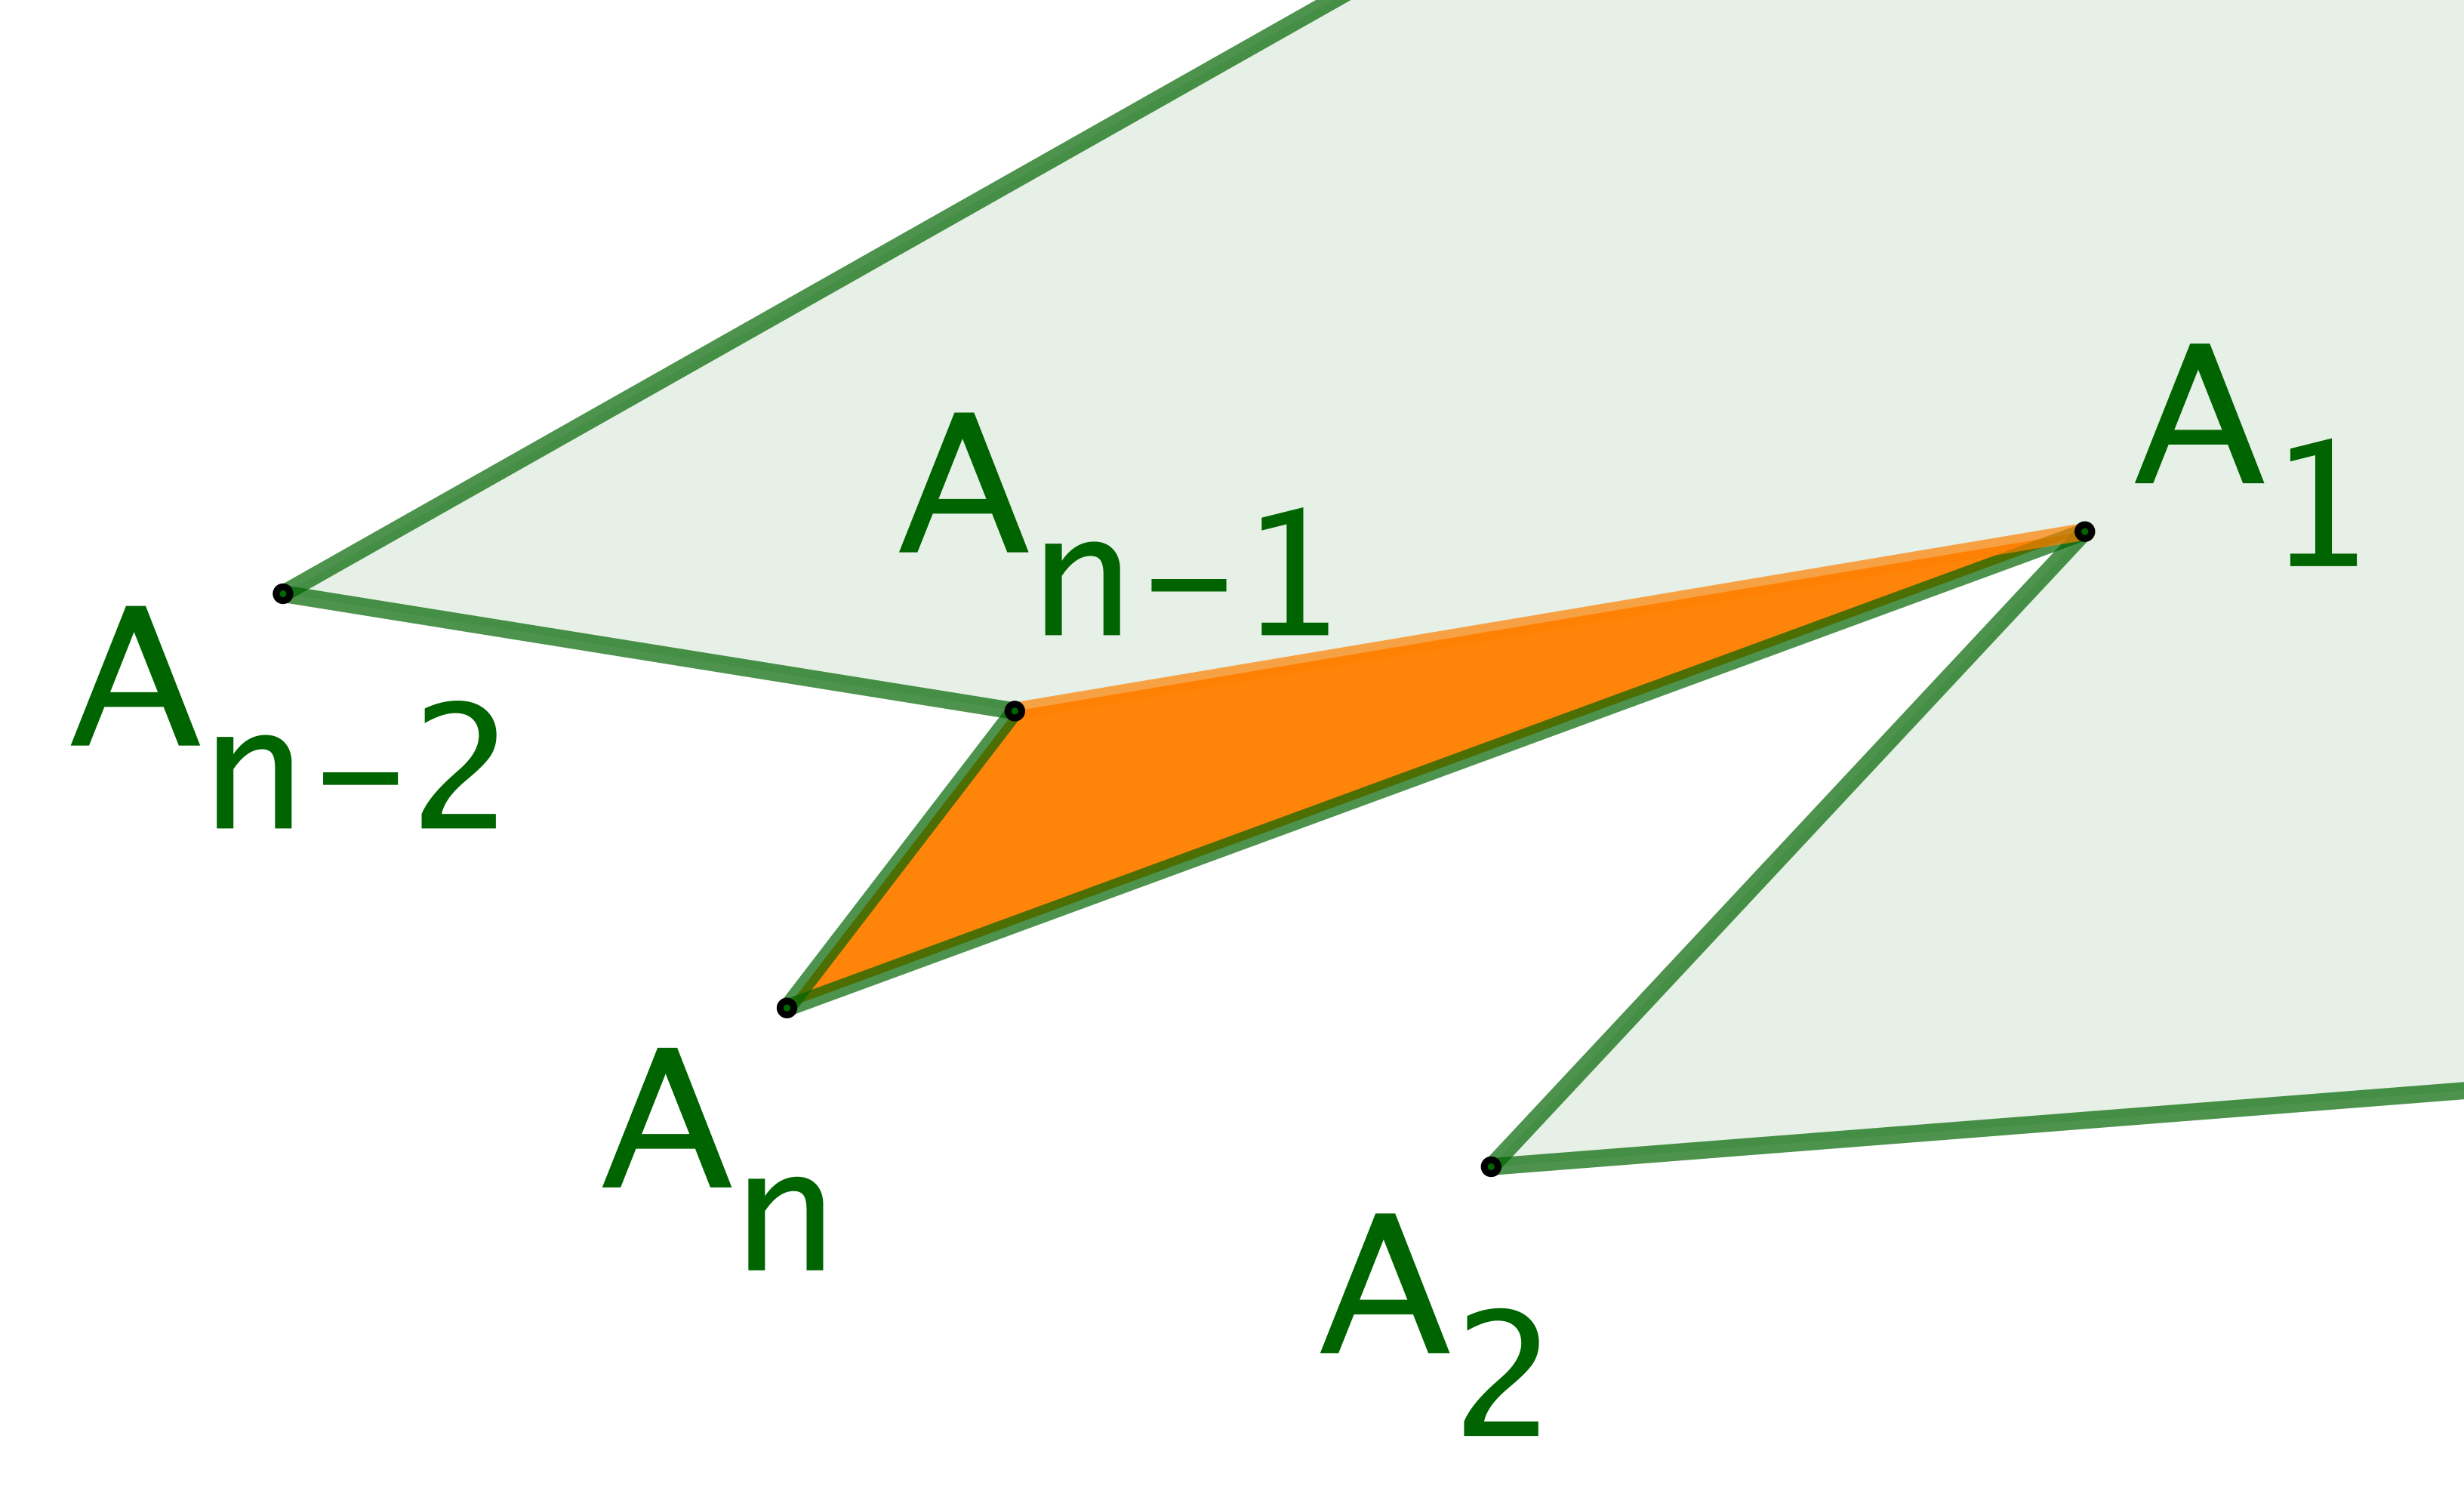
\includegraphics[scale=.4]{content/polygon/at-least-one/triangulation-proof-OK.png}

	        	\smallskip
    	   		$A_{n-1} A_n A_1$ est une oreille.
    	\end{center}

	    	\begin{center}
        	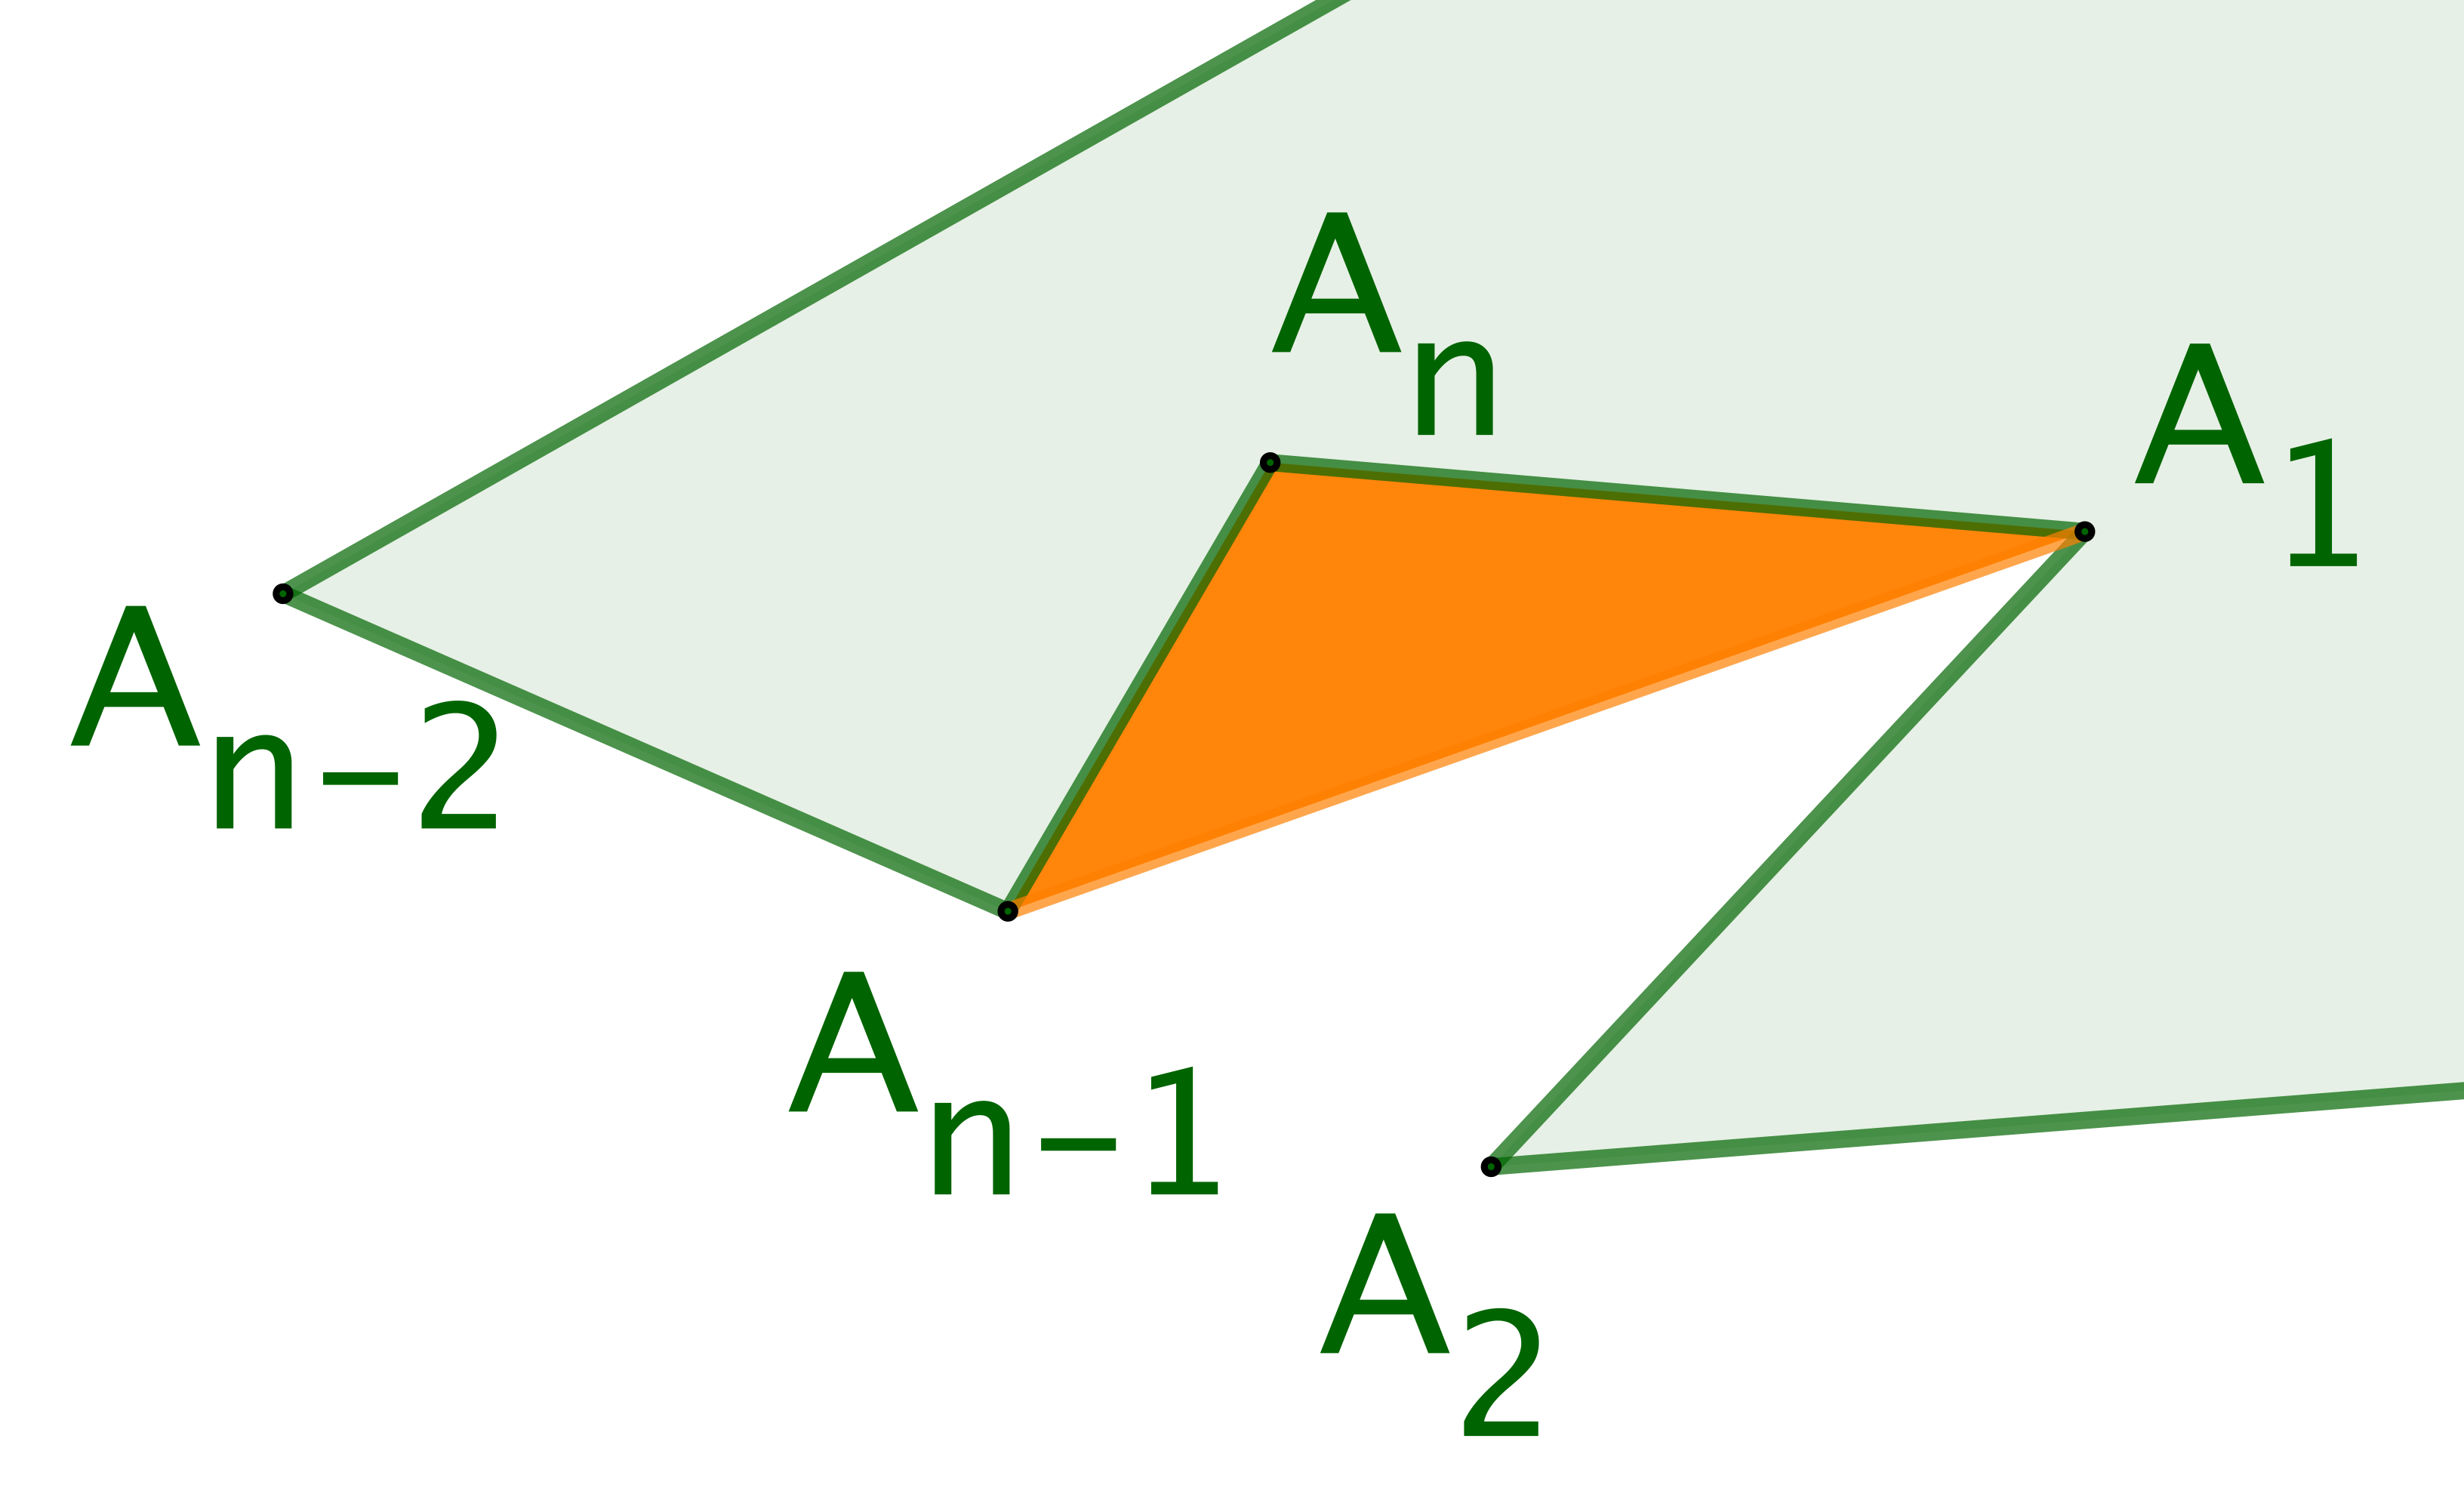
\includegraphics[scale=.4]{content/polygon/at-least-one/triangulation-proof-KO.png}

        		\smallskip
    	   		$A_{n-1} A_n A_1$ n'est pas une oreille.
    		\end{center}
    	\end{multicols}


		\noindent
		Notons $\setproba{P}^{\,\prime}$ le \kgone\ associé au \kcycle\ $\setproba{L}^{\,\prime} = A_1 \cdots A_{n-1}$ où $k = n-1$ vérifie $k \in \NN_{\geq3}$. Par hypothèse, $\setproba{L}^{\,\prime}$ est positive. Nous arrivons aux calculs élémentaires suivants en utilisant $\Omega = A_1$ comme point de calcul de $\mu(\setproba{L})$.

		\leavevmode\kern-2em%
		\begin{stepcalc}[style=ar*]
			\mu(\setproba{L})
		%
%		\explnext{}
%			\dsum_{j=1}^{n} \det \big( \vect{A_1 A^{\,\prime}_j} ,  \vect{A_1 A^{\,\prime}_{j + 1}} \big)
%		%
		\explnext{}
			\dsum_{j=1}^{n-2} \det \big( \vect{A_1 A^{\,\prime}_j} ,  \vect{A_1 A^{\,\prime}_{j + 1}} \big)
			+
			\det \big( \vect{A_1 A^{\,\prime}_{n-1}} ,  \vect{A_1 A^{\,\prime}_n} \big)
			+
			\det \big( \vect{A_1 A^{\,\prime}_n} ,  \vect{A_1 A^{\,\prime}_{n+1}} \big)
		%
		\explnext*{$A_1 = A^{\,\prime}_{n+1}$ \\
		           $A_i = A^{\,\prime}_i$ \\ pour $i \leq n$}%
		          {}
			\dsum_{j=1}^{n-2} \det \big( \vect{A_1 A_j} ,  \vect{A_1 A_{j + 1}} \big)
			+
			\det \big( \vect{A_1 A_{n-1}} ,  \vect{A_1 A_n} \big)
			+
			\det \big( \vect{A_1 A_n} ,  \vect{A_1 A_1} \big)
		%
		\explnext{}
			\dsum_{j=1}^{n-2} \det \big( \vect{A_1 A_j} ,  \vect{A_1 A_{j + 1}} \big)
			+
			\det \big( \vect{A_1 A_{n-1}} ,  \vect{A_1 A_n} \big)
		%
		\explnext{}
			\mu(\setproba{L}^{\,\prime})
			+
			\mu(A_{n-1} A_n A_1)
		\end{stepcalc}


		\noindent
		Par hypothèse de récurrence, nous savons que
		$\mu(\setproba{L}^{\,\prime}) \geq 0$,
		et comme $A_{n-1} A_n A_1$ est une oreille de $\setproba{P}$, la $3$-ligne $A_{n-1} A_n A_1$ est forcément positive, d'où $\mu(A_{n-1} A_n A_1) \geq 0$ d'après le cas de base.
		Nous arrivons bien à $\mu(\setproba{L}) \geq 0$, ce qui permet de finir aisément la démonstration par récurrence.
	\end{itemize}
\end{proof}


% ----------------------- %


\begin{fact} \label{ngone-garea-is-area}
    Pour tout \ngone\ $\setproba{P}$, nous avons: $\garea{\setproba{P}} = \area{\setproba{P}}$.
\end{fact}


\begin{proof}
    Les deux points suivants permettent de faire une preuve par récurrence.

    \begin{itemize}
		\item \textbf{Cas de base.}
		L'égalité est immédiate pour les triangles (c'est ce qui a motivé la définition de l'aire généralisée).


		\item \textbf{Hérédité.}
		Reprenons les notations de la démonstration du fait \ref{route-direction} : $\setproba{P}$ est un \ngone\ , avec $n \in \NN_{>3}$, $\setproba{L} = A_1 A_2 \cdots A_n$ un \ncycle\ positif qui lui est associée, $A_{n-1} A_n A_1$ une oreille d'une triangulation à l'écoute du \ngone\ $\setproba{P}$, $\setproba{P}^{\,\prime}$ le \kgone\ associé au \kcycle\ $\setproba{L}^{\,\prime} = A_1 \cdots A_{n-1}$ où $k = n-1$ vérifie $k \in \NN_{\geq3}$, avec $\setproba{L}^{\,\prime}$ positive. Nous arrivons aux calculs élémentaires suivants.
		
		\newpage
		
		\leavevmode\kern-2em%
		\begin{stepcalc}[style=ar*]
			\area{\setproba{P}}
		%
		\explnext*{$A_{n-1} A_n A_1$ est une oreille de $\setproba{P}$.}%
		          {}
		    \area{\setproba{P}^{\,\prime}} + \area{A_{n-1} A_n A_1}
		%
		\explnext*{Hypothèse de récurrence et cas de base.}%
		          {}
		    \garea{\setproba{P}^{\,\prime}} + \garea{A_{n-1} A_n A_1}
		%
		\explnext*{Voir le fait \ref{route-direction}.}%
		          {}
		    \frac12 \big( \mu(\setproba{L}^{\,\prime}) + \mu(A_{n-1} A_n A_1) \big)
		%
		\explnext*{Comme dans la preuve du fait \ref{route-direction}.}%
		          {}
		    \frac12 \mu(\setproba{L})
		%
		\explnext*{Voir le fait \ref{route-direction}.}%
		          {}
		    \garea{\setproba{P}}
		\end{stepcalc}
    \end{itemize}
\end{proof}


% ----------------------- %


%\newpage

Avant d'avancer, nous devons mieux comprendre le calcul de $\garea{\setproba{L}}$ pour un \ncycle\ $\setproba{L}$ correspondant à un polygone croisé.
Considérons le figure suivante produite via \geogebra, ce dernier donnant les valeurs indiquées sur l'image où l'on constate que $\num{6.88} - \num{2.63} + \num{4.95} = \num{9.2}$.


\begin{center}
    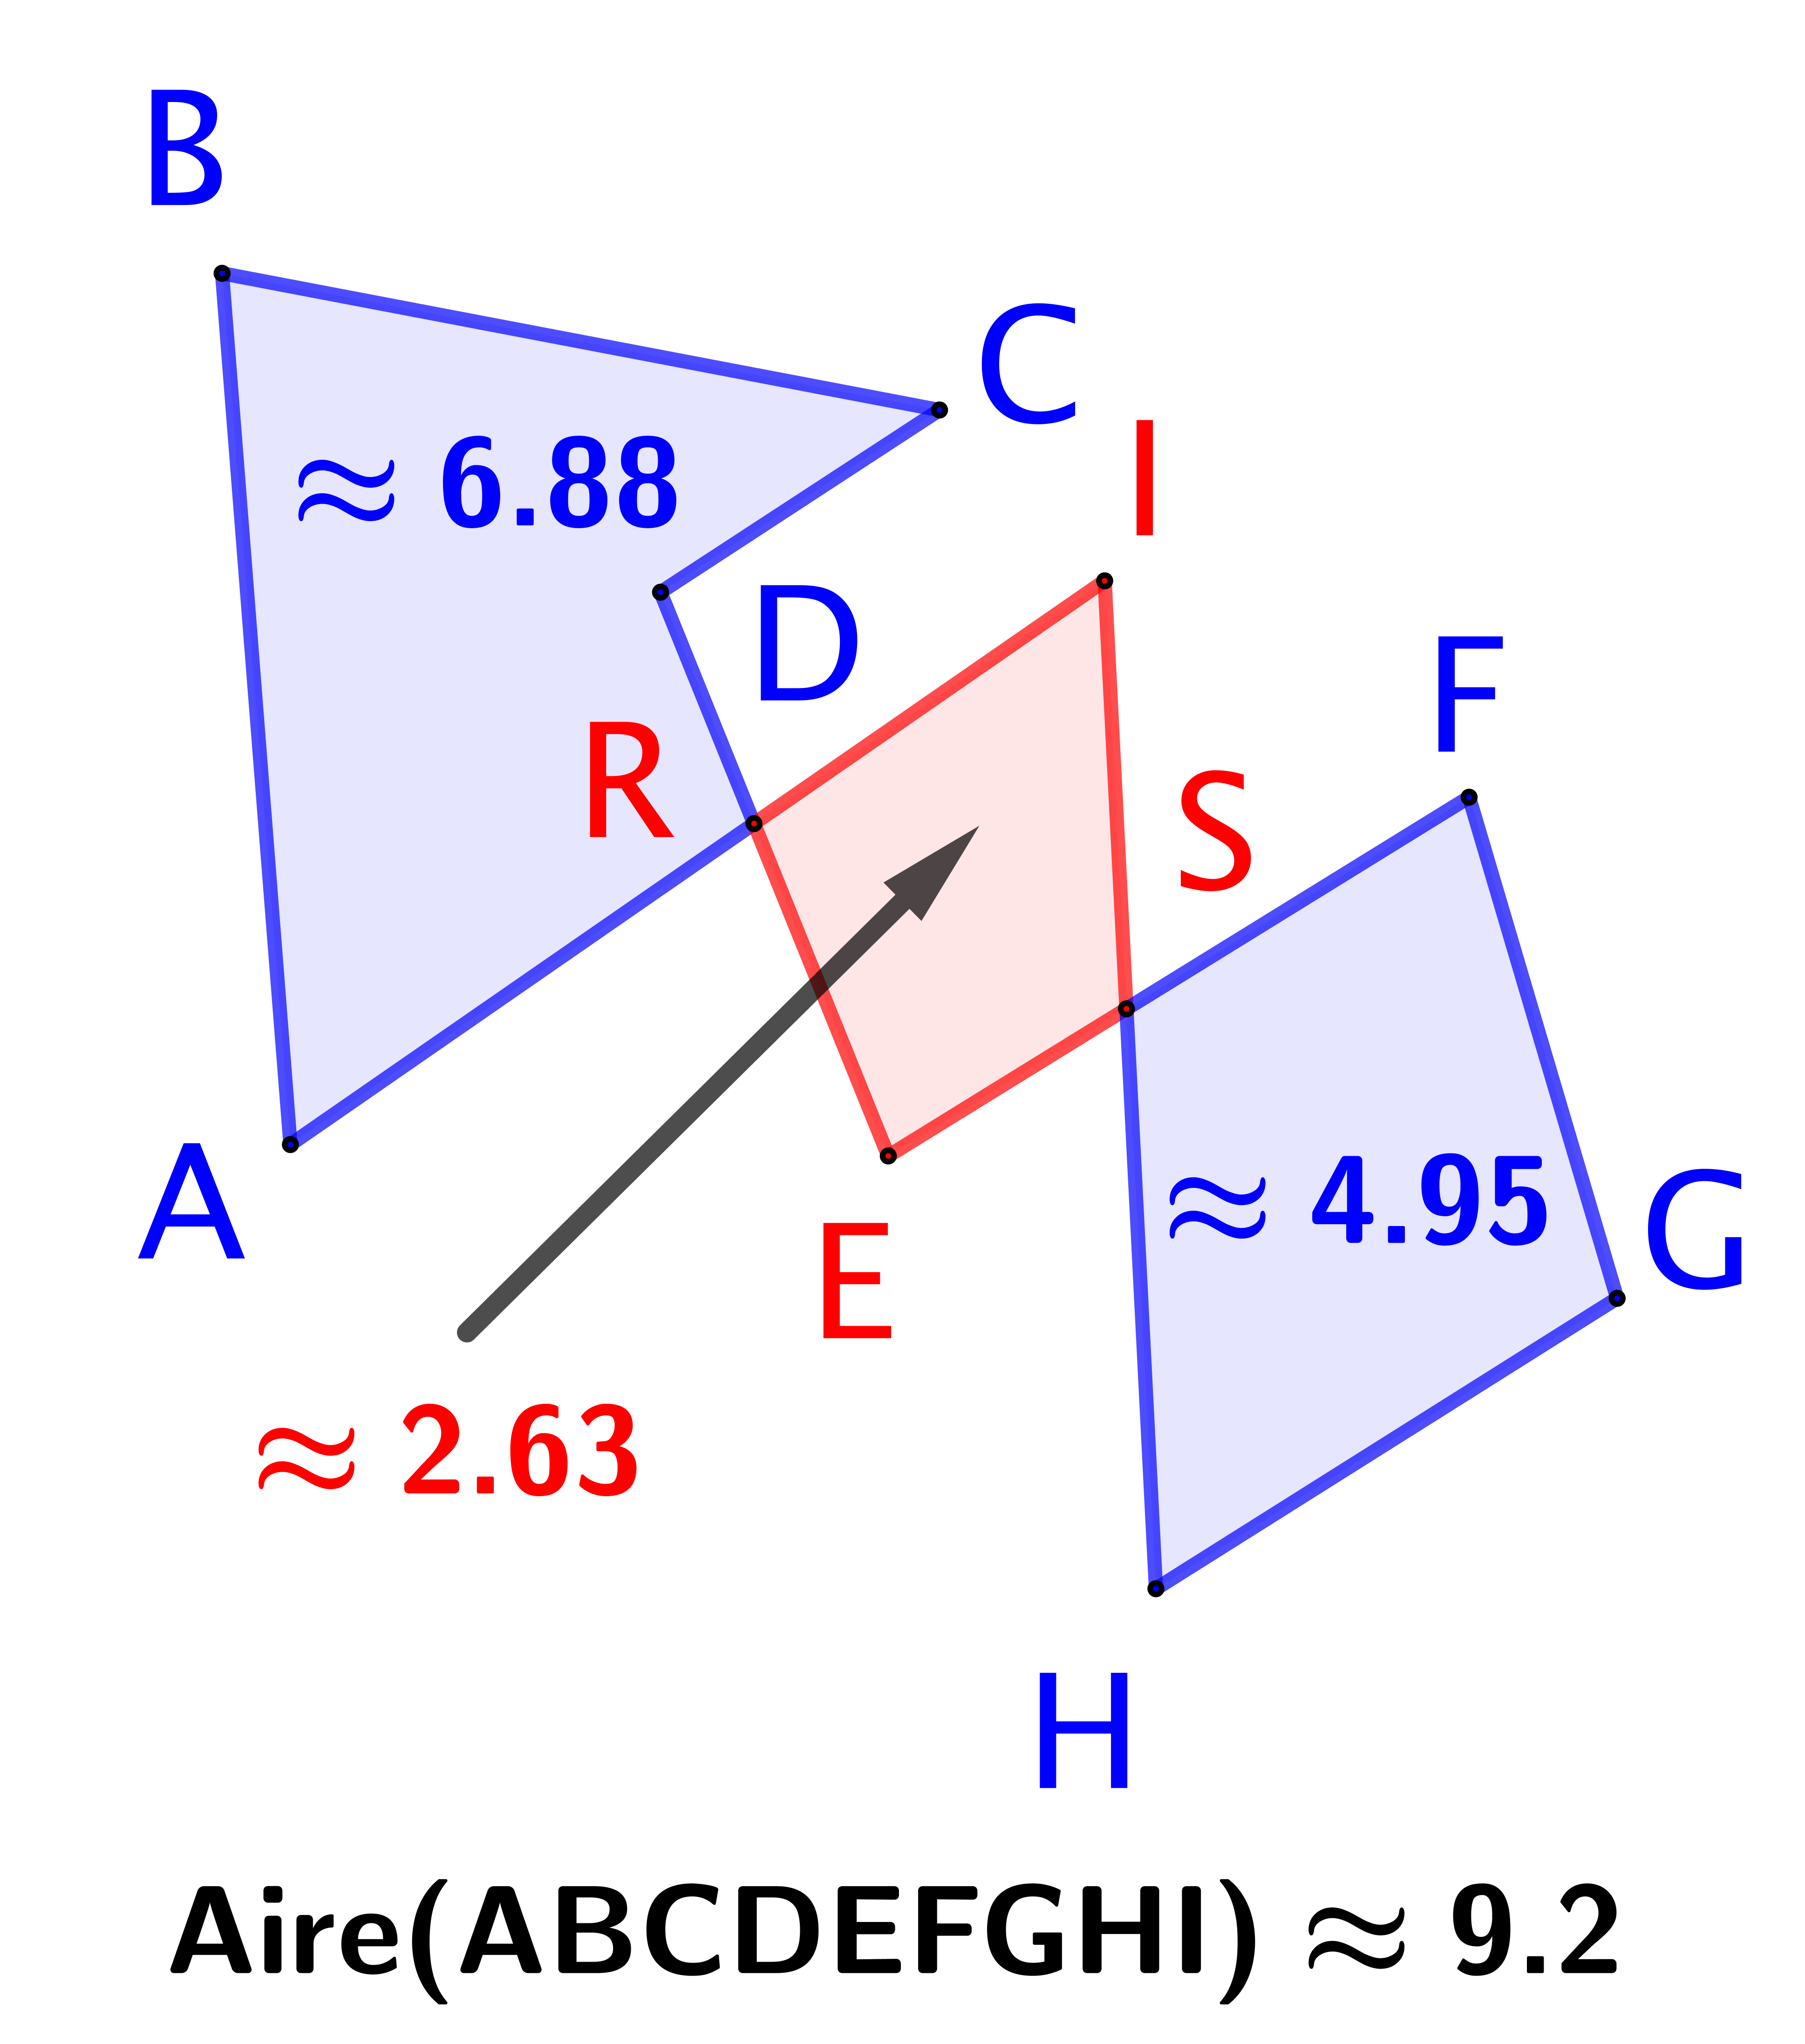
\includegraphics[scale=.35]{content/polygon/at-least-one/garea-trick.png}
\end{center}


Pour calculer l'aire généralisée d'un polygone croisé associé au \ncycle\ $\setproba{L}$, il suffit de procéder comme suit (cette méthode est utile pour un humain).
%
\begin{itemize}
    \item On part d'un point, puis on parcourt le \ncycle\ dans un sens donné jusqu'à la première intersection croisée. Dans notre exemple, on va de $A$ à $R$.

    \item De cette intersection, on change de direction pour choisir celle allant vers notre point de départ. Dans notre exemple, nous obtenons le \kcycle\ $ABCDR$.

    \item Le reste des points non parcourus fournit un autre \kcycle\ qui est $REFGHI$ dans notre cas. Formellement, nous avons scindé $ABCDEFGHI$ en $ABCDR$ et $REFGHI$.

    \item On répète ce processus avec les sous \kcycles\ obtenus jusqu'à n'avoir que des \kgones. Pour notre exemple, nous avons trois \kgones\ $ABCDR$, $RESI$ et $SFGH$.

    \item Les \kgones\ obtenus sont ordonnés en respectant l'ordre du \ncycle\ initial.

    \item Le calcul de l'aire généralisée se fait en ajoutant les aires des \kgones\ de rang impair, puis en retirant celles des \kgones\ de rang pair. En appliquant la valeur absolue au résultat obtenu, nous obtenons l'aire généralisée du polygone croisé initial. Dans notre exemple, nous devons calculer $\abs{ \area{ABCDR} - \area{RESI} + \area{SFGH} }$.
\end{itemize}

Pourquoi cela fonctionne-t-il ? 
Il suffit de revenir à la définition de $\mu(\setproba{L})$ pour constater qu'une règle de type Chasles existe, et de plus qu'en utilisant un point d'intersection de deux arêtes pour un calcul effectif de $\mu(\setproba{L})$, nous avons un changement de sens de parcours du point de vue de ce point d'intersection, ceci justifiant les changements de signe de notre recette, qui n'en est plus une.
Pour le cas suivant, notre approche, plus combinatoire que géométrique, donne $\num{12.26} - \num{1.96} = \num{10.3}$ comme attendu.

%\newpage

\begin{multicols}{2}
	\foreach \n in {1,3,2,4} {
		\begin{center}
    		\includegraphics[scale=.35]{content/polygon/at-least-one/garea-trick-bis-\n.png}
		\end{center}
	}
\end{multicols}


% ----------------------- %


\begin{fact} \label{no-cross-max}
    Si un \ncycle\ $\setproba{L}$ non dégénéré n'est pas un \ngone, donc est un polygone croisé, alors il existe un \ngone\ convexe $\setproba{P}$ tel que
	$\perim{\setproba{P}} = \perim{\setproba{L}}$
	et
	$\garea{\setproba{P}} > \garea{\setproba{L}}$.
\end{fact}


\begin{proof}
	Notons $\setproba{C}$ l'enveloppe convexe de $\setproba{L}$. La méthode de calcul de $\garea{\setproba{L}}$ exposée ci-dessus donne sans ambiguïté que $\garea{\setproba{C}} > \garea{\setproba{L}}$. De plus, il est clair que $\perim{\setproba{C}} < \perim{\setproba{L}}$, mais nous savons juste que $\setproba{C}$ est un \kgone\ avec $k < n$. 
	%
	Comment gérer ce problème?
	%
	Une idée simple, formalisée après, consiste à ajouter des sommets suffisamment prêts des côtés de $\setproba{C}$ pour garder la convexité, un périmètre strictement inférieur à $\perim{\setproba{L}}$, et une aire généralisée strictement plus grande que $\garea{\setproba{L}}$. Si cela est faisable, un agrandissement de rapport $r > 1$ ramènera au périmètre $\perim{\setproba{L}}$ avec une aire strictement plus grande que $\garea{\setproba{L}}$.
	La figure suivante illustre cette idée.

	\begin{center}
		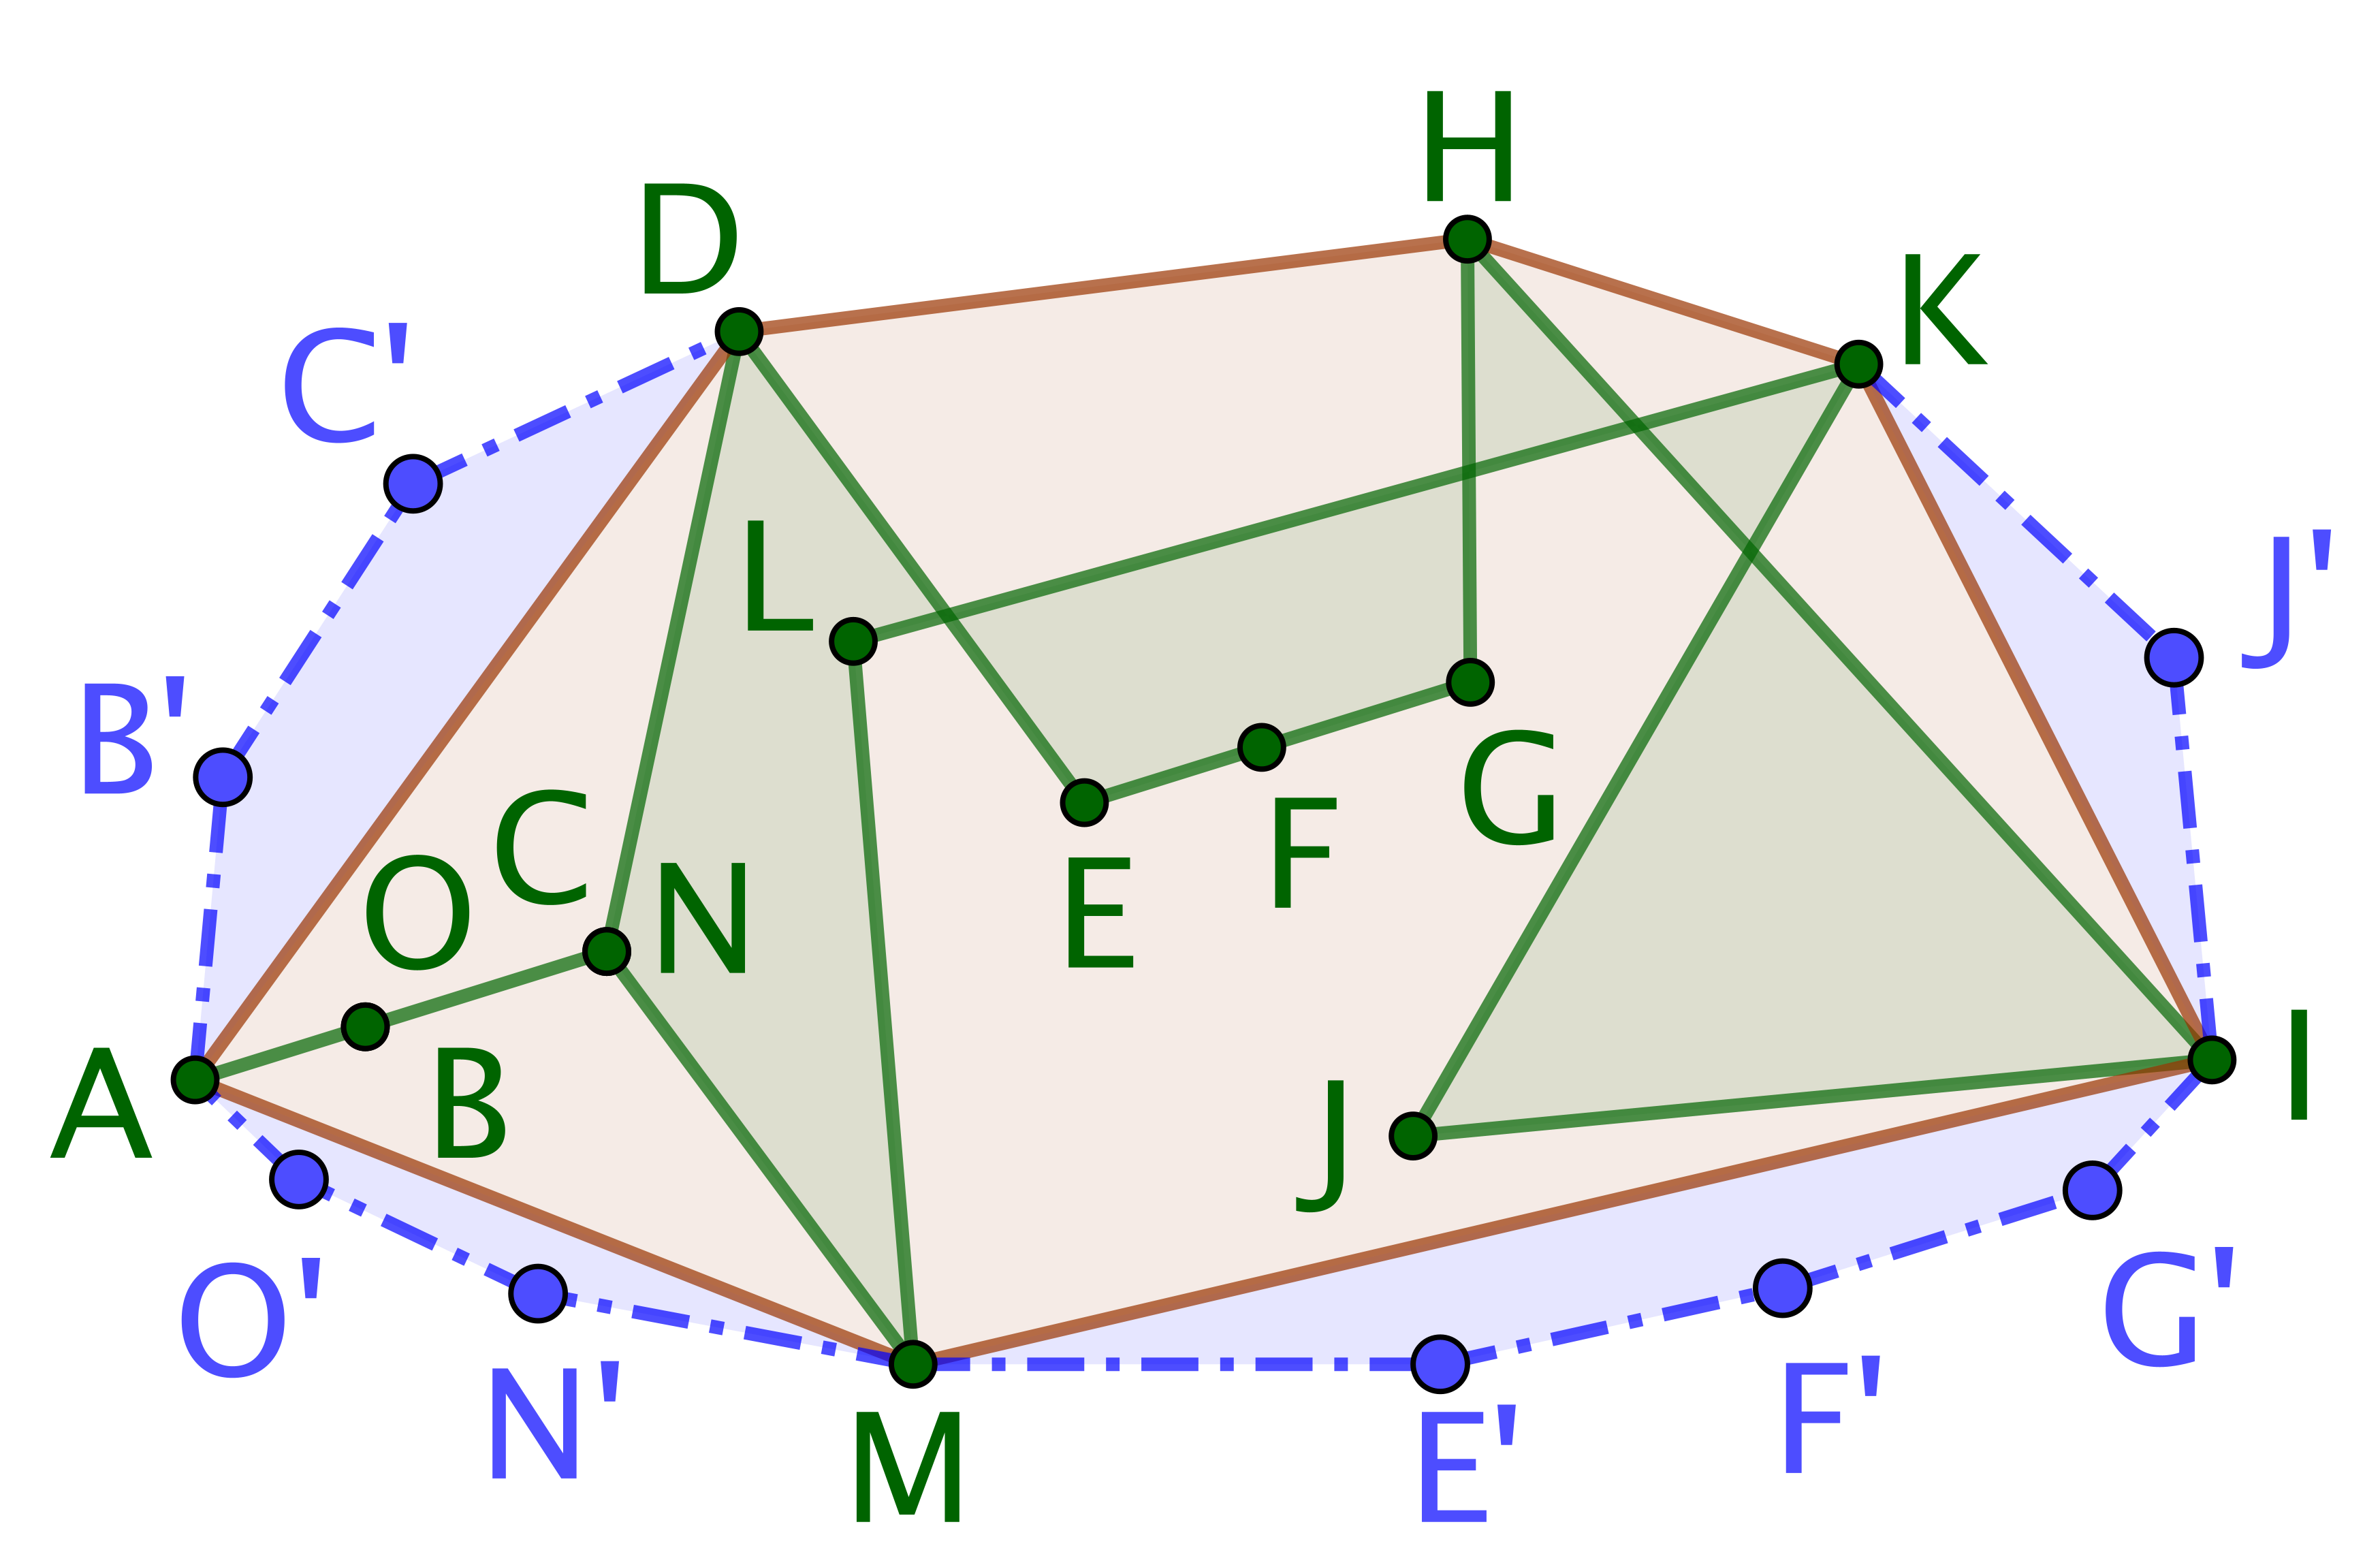
\includegraphics[scale=.4]{content/polygon/at-least-one/convex-hull-distortion.png}
	\end{center}


	Notons $s$ le nombre de sommets dans $\setproba{C}$, nous notons $m = n - s$ le nombre de sommets manquants.
	Si $m = 0$, il n'y a rien à faire.
	Sinon, posons $\delta = \frac{\perim{\setproba{L}} - \perim{\setproba{C}}}{m}$.
	%
	\begin{enumerate}
		\item \label{add-vertex-start}
		Considérons $[AB]$ un côté quelconque de $\setproba{C}$.
		Les droites portées par les côtés \og \emph{autour} \fg\ de $[AB]$ \og \emph{dessinent} \fg\ une région contenant toujours un triangle $ABC$ dont l'intérieur est à l'extérieur
		\footnote{
			C'est ce que l'on appelle de la \og \emph{low poetry} \fg\,.
		}
		de $\setproba{C}$ comme dans les deux cas ci-dessous.
	%
		\begin{multicols}{2}
			\centering

			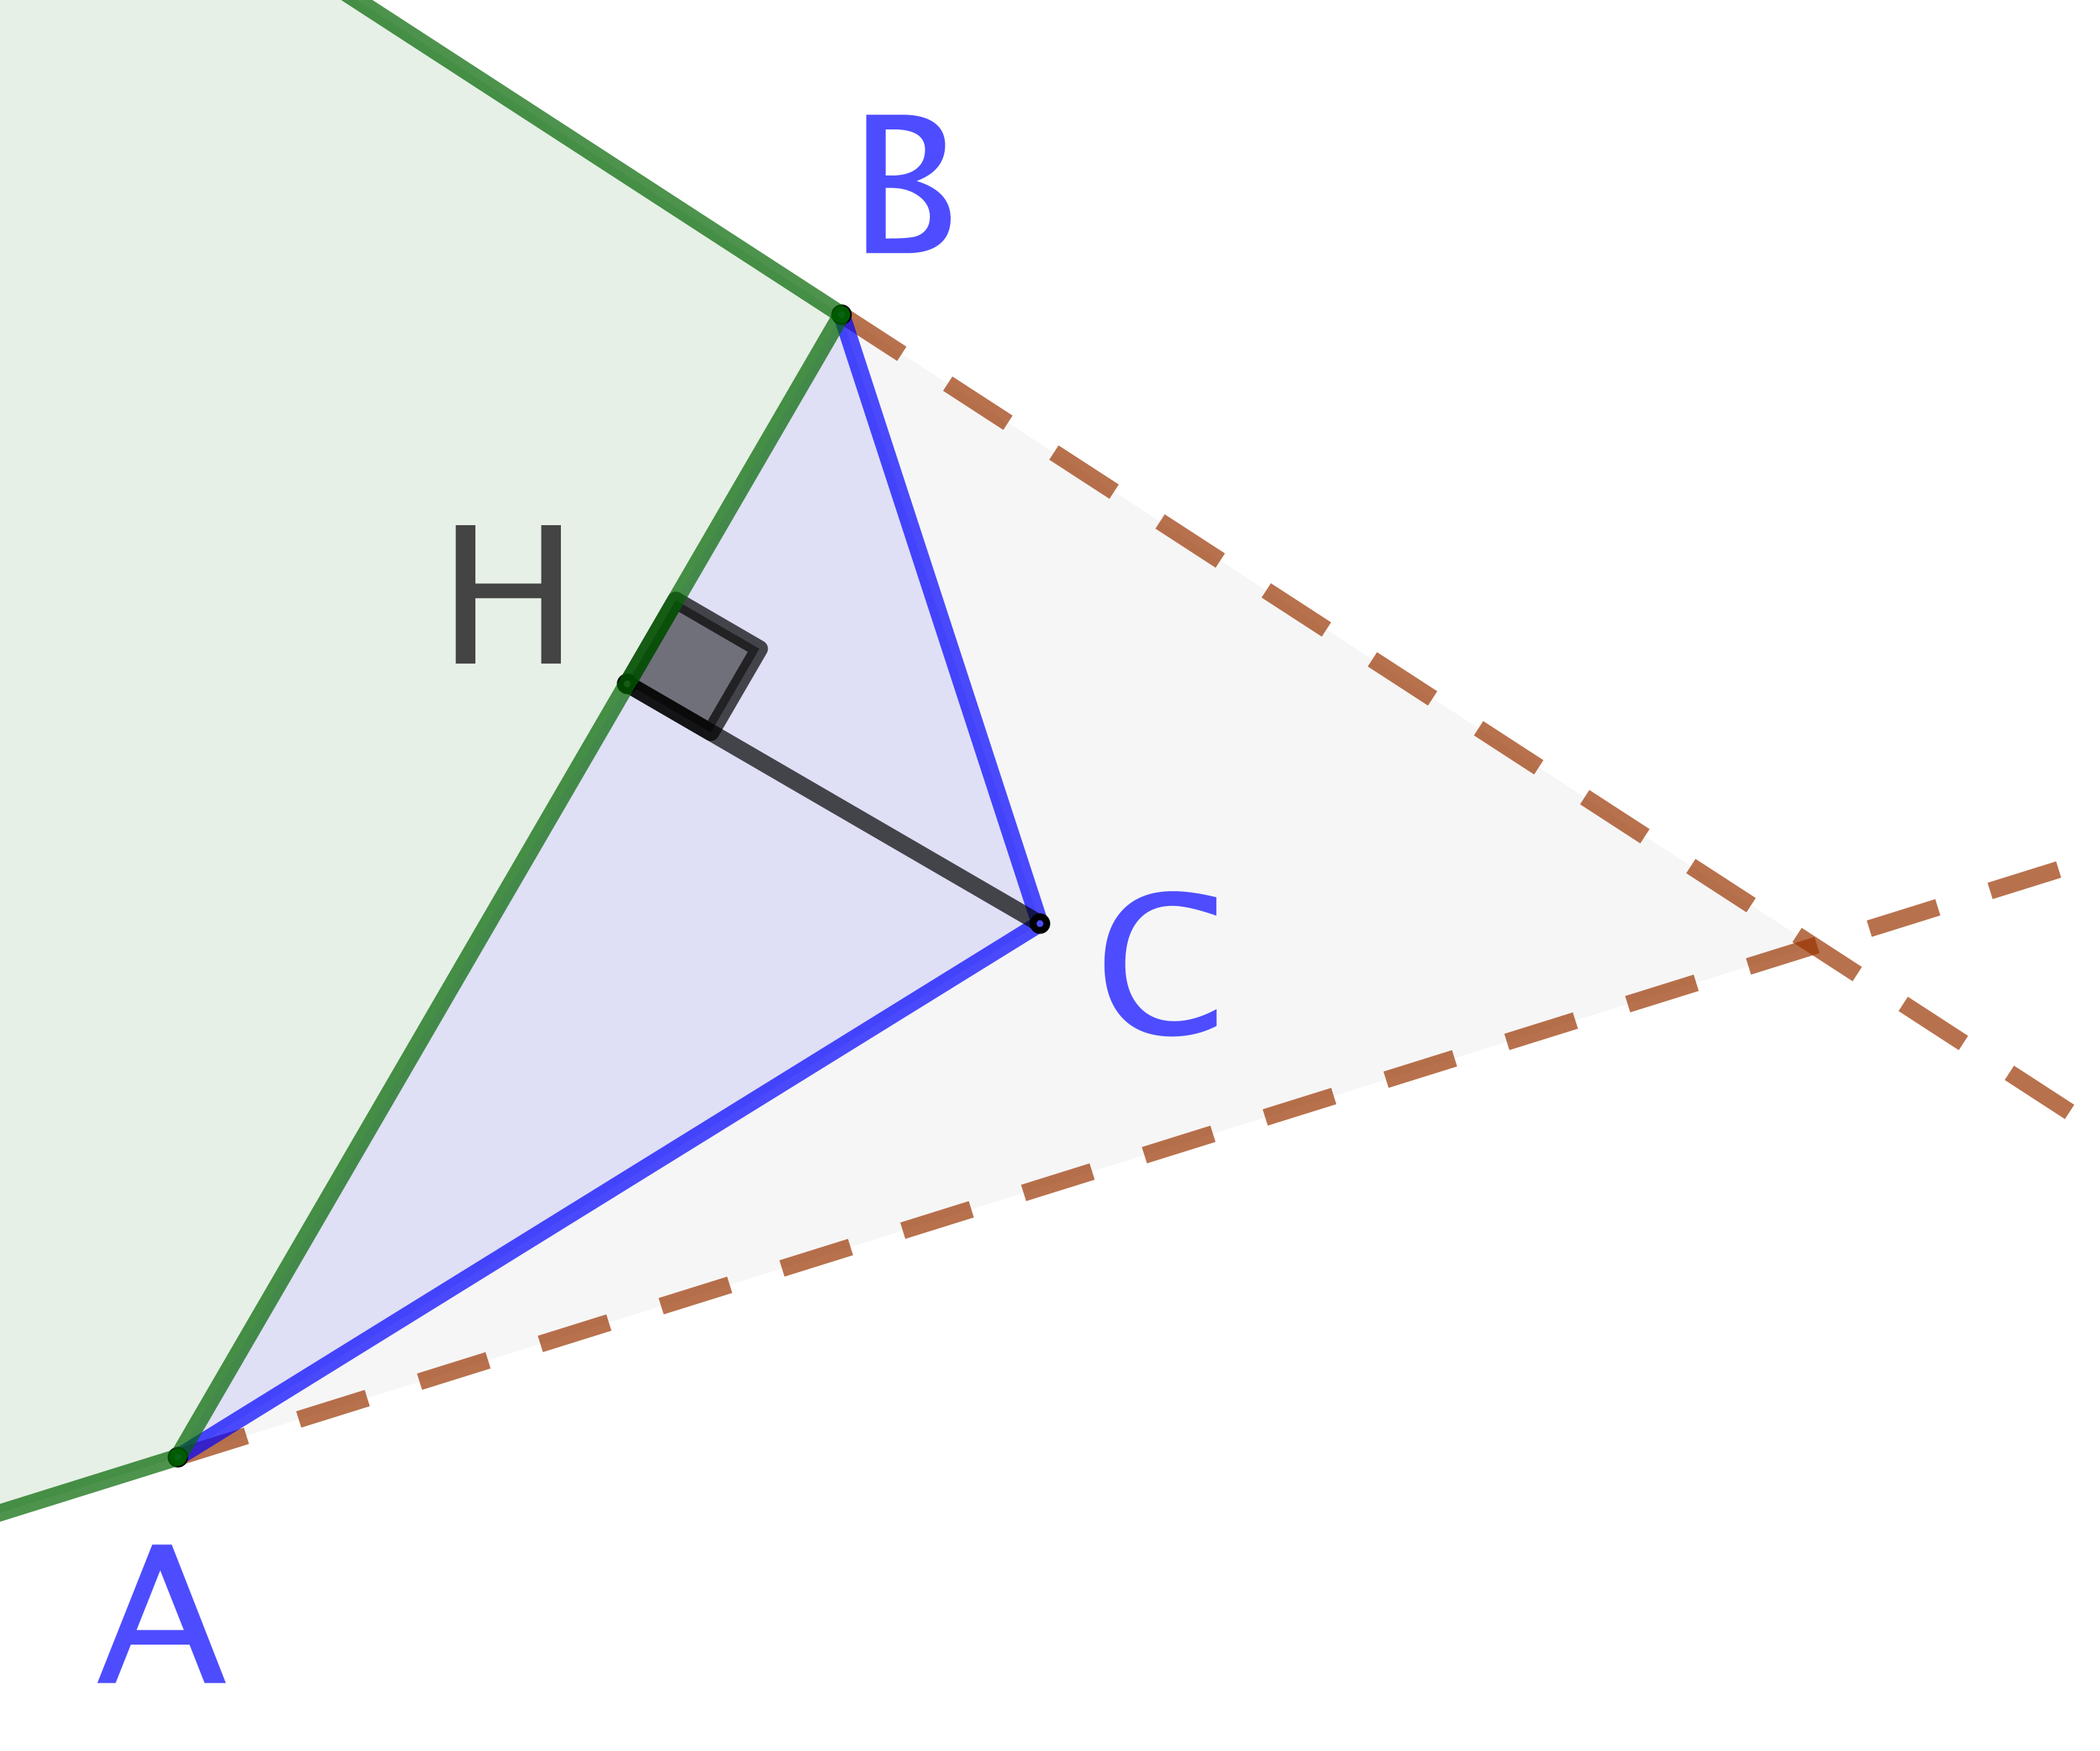
\includegraphics[scale=.4]{content/polygon/at-least-one/add-vertex-1.png}

			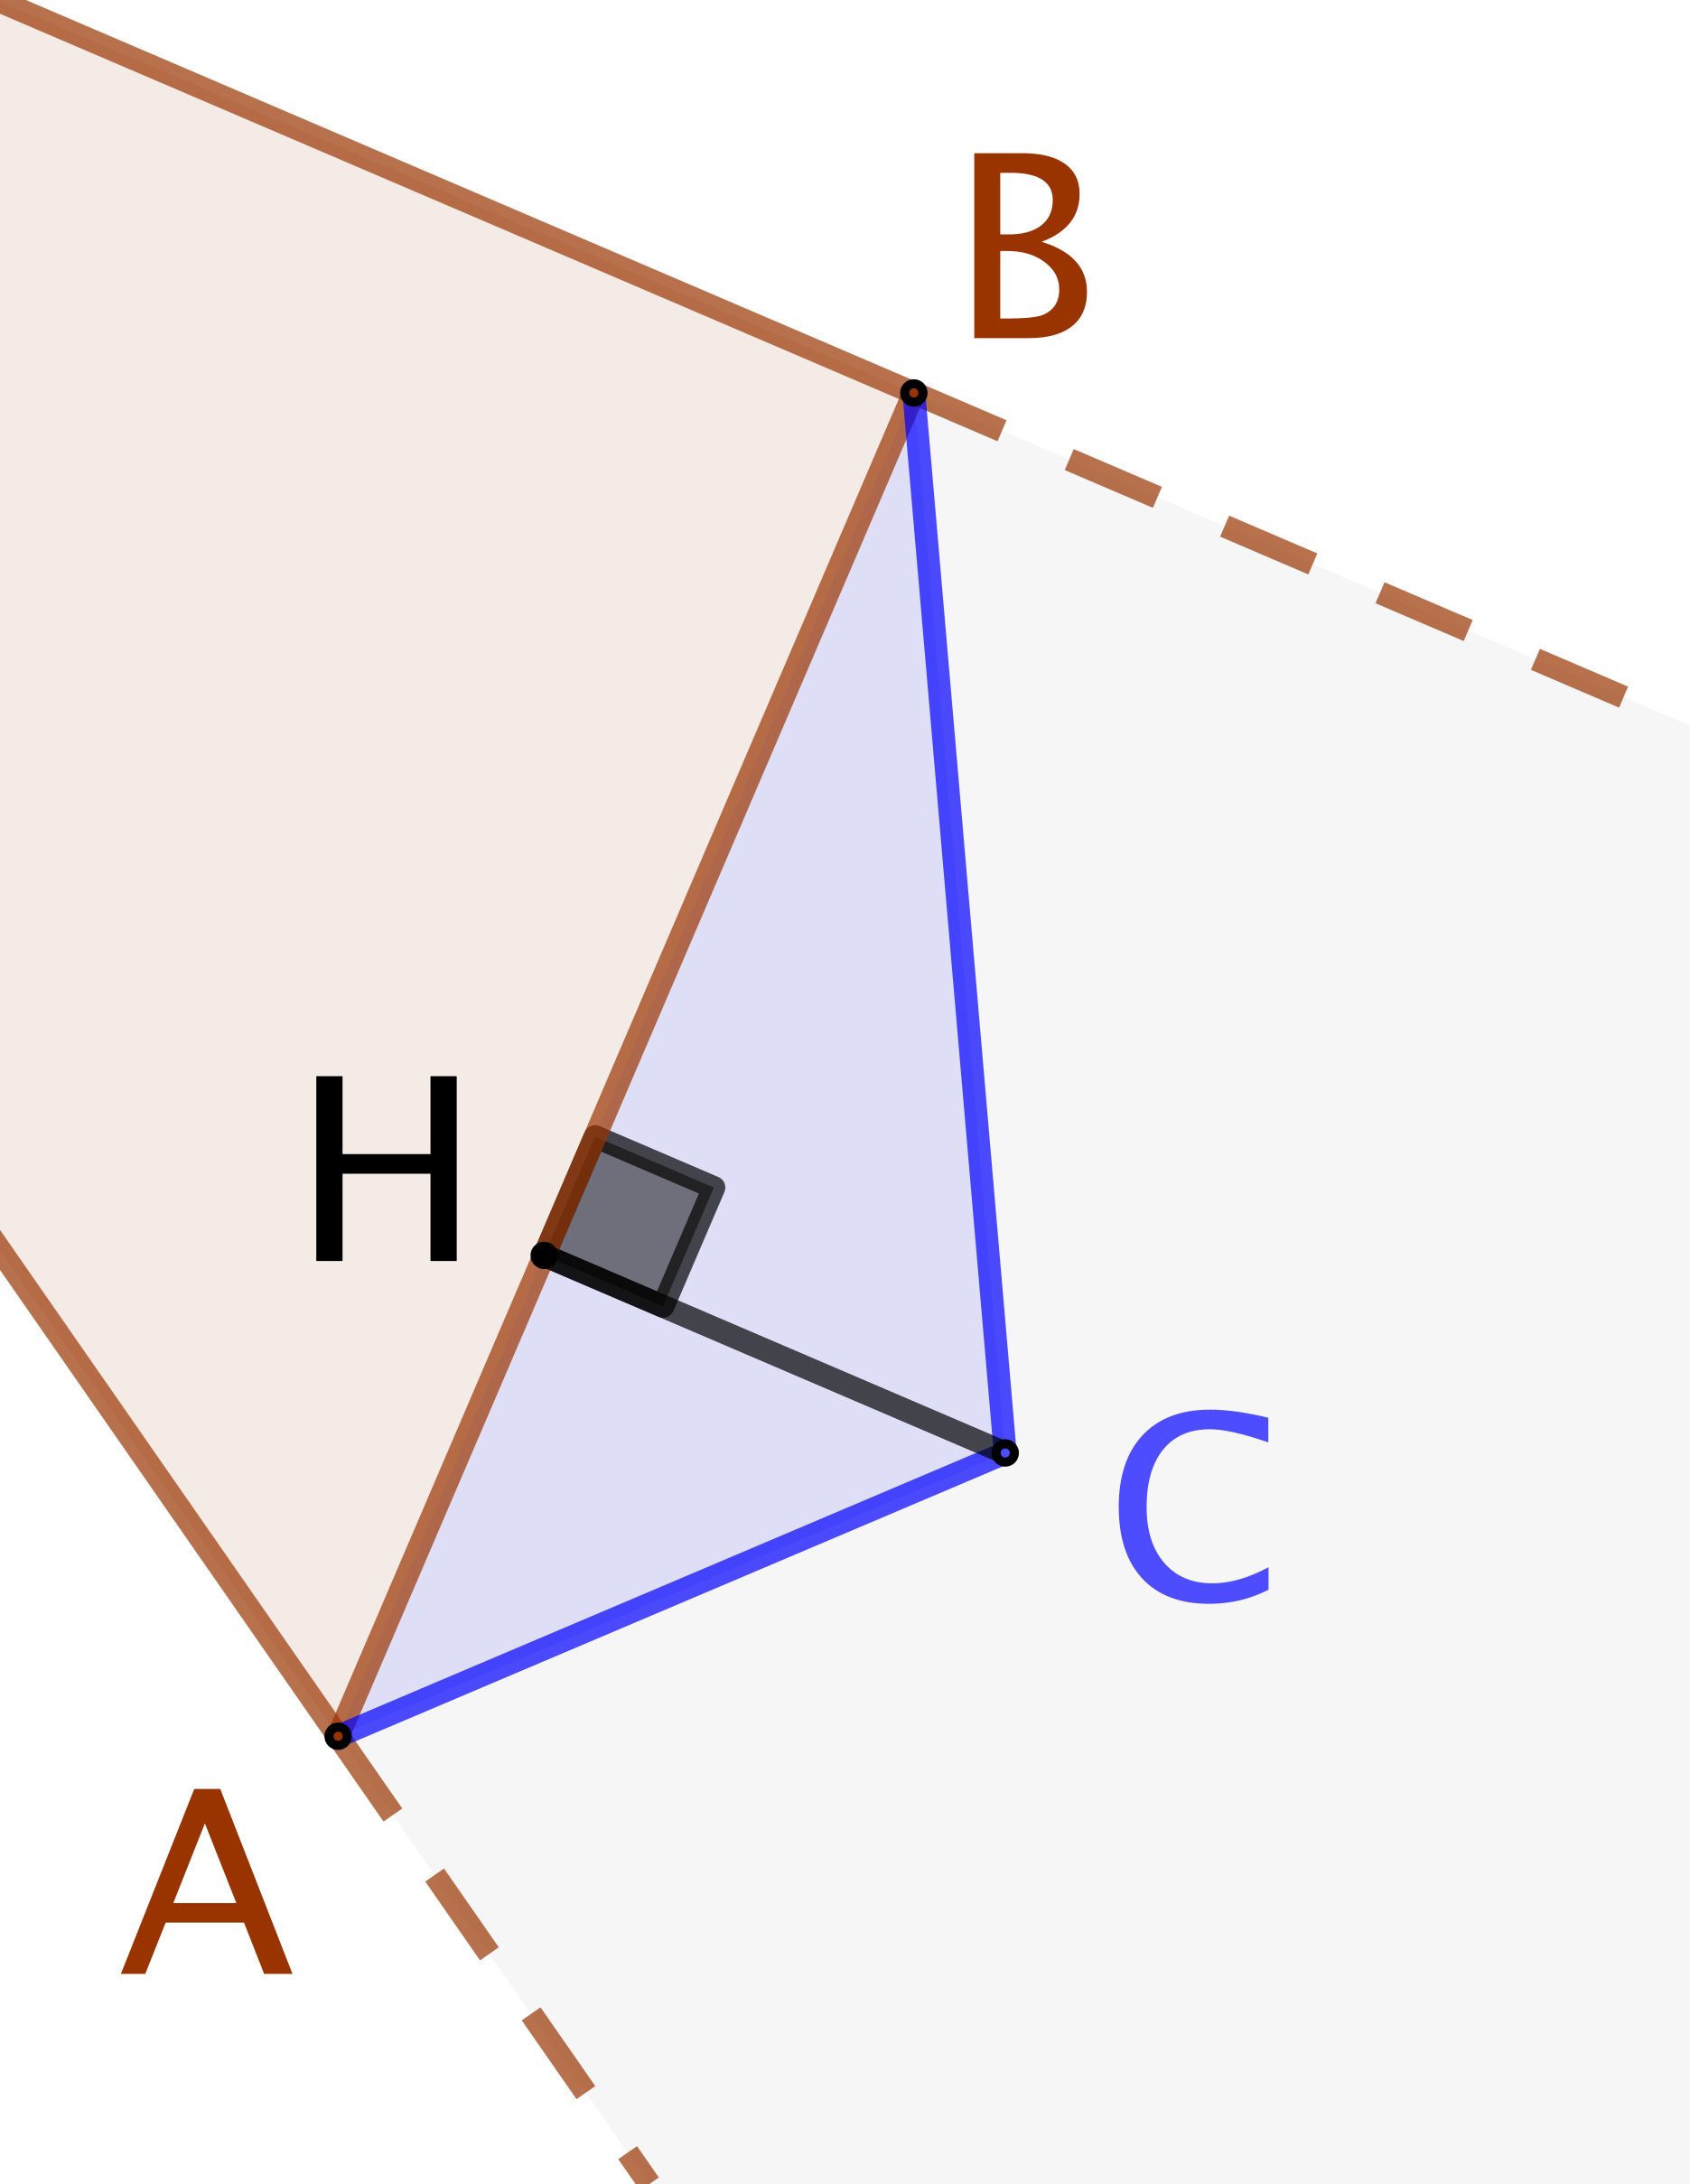
\includegraphics[scale=.4]{content/polygon/at-least-one/add-vertex-2.png}
		\end{multicols}

		\item Clairement, le polygone $\setproba{C}_+$ obtenu à partir de $\setproba{C}$ en remplaçant le côté $[AB]$ par les côtés $[AC]$ et $[CB]$ est un convexe avec un sommet de plus que $\setproba{C}$.

		\item \label{add-vertex-end}
		Comme $HC$ peut être rendu aussi proche de $0$ que souhaité, il est aisé de voir que l'on peut choisir cette distance de sorte que $AC + BC < AB + \delta$.
		Dès lors, le périmètre de $\setproba{C}_+$ augmente inférieurement strictement à $\delta$ relativement à $\setproba{C}$.

		\item En répétant $(m-1)$ fois les étapes \ref{add-vertex-start} à \ref{add-vertex-end}, nous obtenons un \ngone\ convexe $\setproba{C}^{\,\prime}$ tel que
		$\area{\setproba{C}^{\,\prime}} > \area{\setproba{L}}$
		et
		$\perim{\setproba{C}^{\,\prime}} < \perim{\setproba{C}} + m \delta = \perim{\setproba{L}}$.
	\end{enumerate}
\end{proof}


% ----------------------- %


\begin{fact} \label{suff-cond}
    Soit $n \in \NN_{\geq3}$ un naturel fixé.
    Parmi tous les \ncycles\ de périmètre fixé, il en existe au moins un d'aire généralisée maximale, un tel \ncycle\ devant être forcément un \ngone.
\end{fact}


\begin{proof}
	Notons $p$ le périmètre fixé..
	%
    \begin{itemize}
        \item Munissant le plan d'un repère orthonormé direct $\pvaxes{O | i | j}$, on note $\setproba{Z}$ l'ensemble des \ncycles\ $\setproba{L} = A_1 A_2 \cdots A_n$ tels que
        $\perim{A_1 A_2 \cdots A_n} = p$
        et
        $A_1\coord{0 | 0}$,%
        \footnote{
        	Le mot \og \emph{Zeile} \fg\ est une traduction possible de \og \emph{ligne} \fg\ en allemand.
        }
        puis $\setproba{G} \subset \RR^{2n}$ l'ensemble des uplets de coordonnées $\big( x(A_1) ; y(A_1) ; \dots ; x(A_n) ; y(A_n) \big)$ pour $A_1 A_2 \cdots A_n \in \setproba{Z}$.


        \item $\setproba{G}$ est clairement fermé dans $\RR^{2n}$.
        De plus, il est borné, car les coordonnées des sommets des \ncycles\ considérés le sont.
        En résumé, $\setproba{G}$ est un compact de $\RR^{2n}$.


        \item Nous définissons la fonction $\alpha: \setproba{G} \rightarrow \RRp$ qui à un uplet de $\setproba{G}$ associe l'aire généralisée du \ncycle\ qu'il représente.
        Cette fonction est continue comme valeur absolue d'une fonction polynomiale en les coordonnées.


        \item Finalement, par continuité et compacité, on sait que $\alpha$ admet un maximum sur $\setproba{G}$.
        Or, un tel maximum ne peut pas être atteint en un \ncycle\ dégénéré, clairement, ni en un polygone croisé d'après le fait \ref{no-cross-max}, donc un tel maximum sera obtenu en un \ngone. That's all folks!
    \end{itemize}
\end{proof}
